% Copyright (C) 2013 - EDF R&D - Michael Baudin

\documentclass{beamer}

% Copyright (C) 2012 - 2013 - EDF R&D - Michael Baudin

\setbeameroption{hide notes}
%\setbeameroption{show notes}
%\setbeameroption{show only notes}
%\mode<presentation>{\usetheme{EDF09}}

% Configuration beamer
\usetheme{Montpellier}
\setbeamertemplate{navigation symbols}{} % Remove navigation
\useoutertheme{infolines}
\setbeamertemplate{theorems}[numbered] 
% Utilise des fonts serif, pour �viter les pb de fonte
\usefonttheme{serif} 
\setbeamertemplate{caption}[numbered]


\usepackage[utf8]{inputenc}
\usepackage[T1]{fontenc}


\usepackage[french]{babel}
\uselanguage{French}
\languagepath{French}

% Scilab macros
\newcommand{\sciobj}[1]{\texttt{#1}}
\newcommand{\scifile}[1]{\texttt{#1}}

% Python macros
\newcommand{\pyobj}[1]{\textcolor{blue}{\texttt{#1}}}

\def\RR{\mathbb{R}}
\def\NN{\mathbb{N}}
\def\ZZ{\mathbb{Z}}
\def\bx{{\bf x}}

% To highlight source code
\usepackage{listingsutf8}
\lstset{inputencoding=utf8/latin1}

\definecolor{darkgreen}{rgb}{0,0.5,0}
\definecolor{violet}{rgb}{0.5,0,1}
\lstset{
  % general command to set parameter(s)
   basicstyle=\scriptsize\ttfamily, %
   keywordstyle=\color{violet}\bfseries,%
   commentstyle=\color{darkgreen}\bfseries,%
   showspaces=false,%
   stringstyle=\color{red}\bfseries
}

\hypersetup{
    %bookmarks=true,         % show bookmarks bar?
    %unicode=false,          % non-Latin characters in Acrobat�s bookmarks
    %pdftoolbar=true,        % show Acrobat�s toolbar?
    %pdfmenubar=true,        % show Acrobat�s menu?
    %pdffitwindow=false,     % window fit to page when opened
    %pdfstartview={FitH},    % fits the width of the page to the window
    %pdftitle={My title},    % title
    %pdfauthor={Author},     % author
    %pdfsubject={Subject},   % subject of the document
    %pdfcreator={Creator},   % creator of the document
    %pdfproducer={Producer}, % producer of the document
    %pdfkeywords={keyword1} {key2} {key3}, % list of keywords
    %pdfnewwindow=true,      % links in new window
    colorlinks=true,       % false: boxed links; true: colored links
    %linkcolor=red,          % color of internal links (change box color with linkbordercolor)
    %citecolor=green,        % color of links to bibliography
    %filecolor=magenta,      % color of file links
    urlcolor=blue           % color of external links
}

\title[Validation des logiciels]{Validation des logiciels de calcul numérique probabilistes}

\author[EDF R\&D]{Micha\"el~Baudin}

\institute[]{
EDF R\&D\\ 
6, quai Watier,78401 Chatou\\
michael.baudin@edf.fr
}

\date{Octobre 2013}

%%%%%%%%%%%%%%%%%%%%%%%%%%%%%%%%%%%%%%%%%%%%%%%%%%%%%%%%%%%%%%%%%%%%%%%%%%%%%

  \begin{document}

%%%%%%%%%%%%%%%%%%%%%%%%%%%%%%%%%%%%%%%%%%%%%%%%%%%%%%%%%%%%%%%%%%%%%%%%%%%%%

\begin{frame}[plain]
    \titlepage
%\titlepage
\end{frame}
\setbeamertemplate{background canvas}{}

\note{
\begin{itemize}
\item Bonjour. 
\end{itemize}
}

%%%%%%%%%%%%%%%%%%%%%%%%%%%%%%%%%%%%%%%%%%%%%%%%%%%%%%%%%%%%%%%%%%%%%%%%%%%%%

\begin{frame}
  \begin{columns}
    \column{0.5\textwidth}
    {\usebeamercolor[fg]{title page}\huge{Sommaire}}
    \vspace{1cm}
    \tableofcontents
  \end{columns}
\end{frame}

%%%%%%%%%%%%%%%%%%%%%%%%%%%%%%%%%%%%%%%%%%%%%%%%%%%%%%%%%%%%%%%%%%%%%%%%%%%%%
\section{Introduction}

\begin{frame}[containsverbatim]
\frametitle{Valider, c'est quoi ?}

On valide quoi ? Une \emph{fonction} de calcul :
\begin{center}
(sortie calculée) (est une fonction de) (entrée fournie)
\end{center}

On valide comment ? Par comparaison :
\begin{center}
(sortie calculée) (correspond à) (sortie attendue)
\end{center}

  \begin{columns}
    \column{0.45\textwidth}

Fonction de calcul - exemples :
\begin{itemize}
\item $G(x)=\sin(x)$ où $x\in\RR$
\item $G(x_1,x_2)=x_1+x_2$ où $x_1,x_2\in\RR$
\item $G(\bx)=\textrm{Aster}(\bx)$ où $\bx=(x_1,\ldots,x_n)^T\in\RR^n$ et $n$ est grand.
\end{itemize}

    \column{0.55\textwidth}

\begin{center}
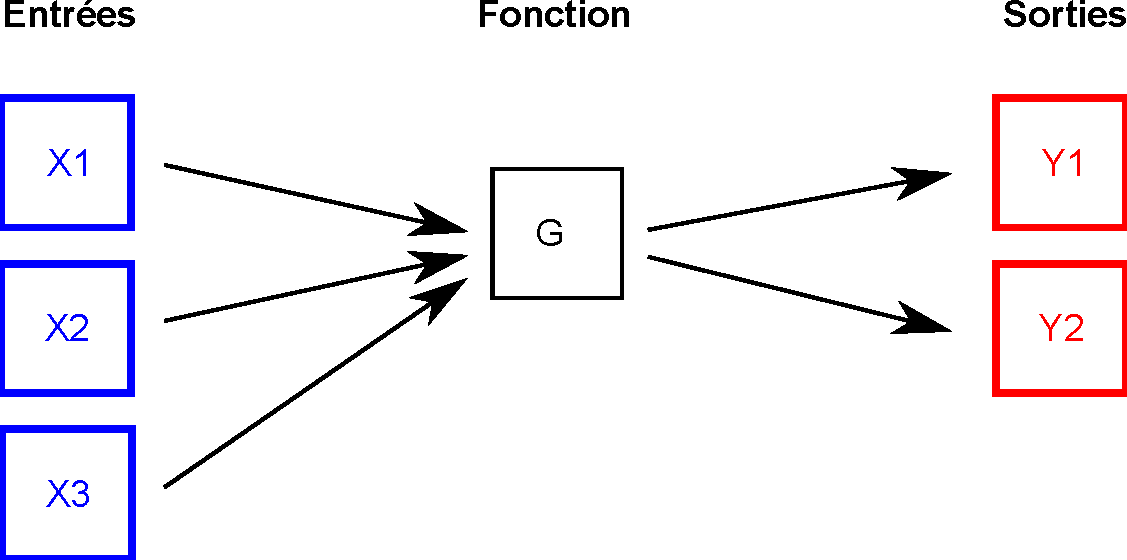
\includegraphics[width=1.\textwidth]{YGX}
\end{center}

	\end{columns}

\end{frame}

%%%%%%%%%%%%%%%%%%%%%%%%%%%%%%%%%%%%%%%%%%%%%%%%%%%%%%%%%%%%%%%%%%%%%%%%%%%%%

\begin{frame}[containsverbatim]
\frametitle{Certes, et après ?}

Objectif :
\begin{enumerate}
\item Valider les résultats de sortie d'un logiciel ...
\item ... de calcul numérique probabiliste.
\end{enumerate}

Partie "logiciel" pure en annexe :
\begin{itemize}
\item Testabilité 
	\begin{itemize}
	\item Améliorer la testabilité d'une fonction, 
	\item la notion de privé/public pour gérer les tests
	\end{itemize}
\item Combinatoire 
	\begin{itemize}
	\item Limiter le nombre de combinaisons d'options à tester, 
	\item choisir ses expériences selon un plan.
	\end{itemize}
\end{itemize}

Généralités \emph{relativement} intuitives : annexe (sur question).

\end{frame}

%%%%%%%%%%%%%%%%%%%%%%%%%%%%%%%%%%%%%%%%%%%%%%%%%%%%%%%%%%%%%%%%%%%%%%%%%%%%%

\begin{frame}[containsverbatim]
\frametitle{Tester un logiciel de calcul}

Partie calcul numérique :
\begin{enumerate}
\item Comparer deux réels en théorie :
	\begin{itemize}
	\item comment est représenté un réel en machine : 
	l'erreur de représentation des nombres flottants,
	\item comment une (petite) erreur en entrée $X$ se transforme en 
	(parfois grande) erreur sur la sortie $Y$ : erreur et conditionnement.
	\end{itemize}
\item Comparer deux réels en pratique :
	\begin{itemize}
	\item comment utiliser une librairie d'assertions numérique 
	pour réaliser un test,
	\item comment tester une fonction probabiliste.
	\end{itemize}
\end{enumerate}

Pas du tout intuitif : c'est le corps de la présentation.

\end{frame}

%%%%%%%%%%%%%%%%%%%%%%%%%%%%%%%%%%%%%%%%%%%%%%%%%%%%%%%%%%%%%%%%%%%%%%%%%%%%%
\section{Flottants}

%%%%%%%%%%%%%%%%%%%%%%%%%%%%%%%%%%%%%%%%%%%%%%%%%%%%%%%%%%%%%%%%%%%%%%%%%%%%%
\begin{frame}
\frametitle{Flottants}
  \begin{columns}
    \column{0.5\textwidth}
    
    \column{0.5\textwidth}
    {\usebeamercolor[fg]{title}\huge{Flottants}}
	
	La différence entre $\RR$ et $\mathcal{F}$.
  \end{columns}
\end{frame}

% %%%%%%%%%%%%%%%%%%%%%%%%%%%%%%%%%%%%%%%%%%%%%%%%%%%%%%%%%%%%%%%%%%%%%%%%%%%%%

% \begin{frame}
% \frametitle{\emph{"Impossible de tester tous les flottants !"}}

% J'ai une fonction $y=G(x)$, où $x$ est un nombre flottant 
% à double précision sur 64 bits.

% Dois-je réaliser $2^{64}$ tests pour valider $G$ ?

% En théorie, oui. 

% Mais en pratique, heureusement, non !

% En revanche, il est utile de savoir ce qu'est un nombre flottant...

% \end{frame}

%%%%%%%%%%%%%%%%%%%%%%%%%%%%%%%%%%%%%%%%%%%%%%%%%%%%%%%%%%%%%%%%%%%%%%%%%%%%%

%\subsection{IEEE-754}

\begin{frame}
\frametitle{Nombres flottants 64 bits}

Un nombre à virgule flottante binaire de type IEEE-754 64 bits :

\begin{center}
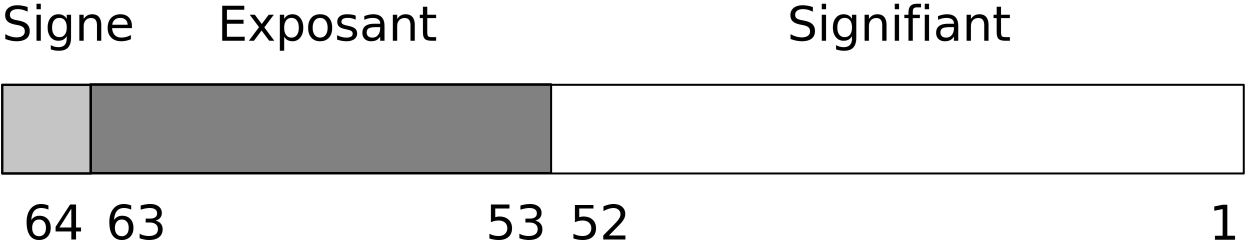
\includegraphics[width=0.8\textwidth]{doubleIEEE754}
\end{center}

Les "doubles" :
\begin{itemize}
\item 1 bit de signe
\item 11 bits d'exposant
\item 53 bits de signifiant (dont 1 implicite)
\end{itemize}

\end{frame}

%%%%%%%%%%%%%%%%%%%%%%%%%%%%%%%%%%%%%%%%%%%%%%%%%%%%%%%%%%%%%%%%%%%%%%%%%%%%%

\begin{frame}
\frametitle{Nombres flottants : principes}

Tous les flottants dans un système "jouet".

\begin{center}
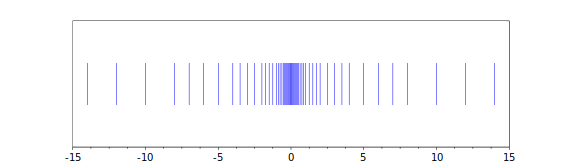
\includegraphics[width=0.9\textwidth]{toysystem_all}
\end{center}

Analogie - Mesure de longueurs sur une règle graduée :
\begin{itemize}
\item qui permet de mesurer des nombres négatifs
\item qui a une longueur finie
\item dont les graduations sont plus resserées autour de zéro
\end{itemize}

\end{frame}

%%%%%%%%%%%%%%%%%%%%%%%%%%%%%%%%%%%%%%%%%%%%%%%%%%%%%%%%%%%%%%%%%%%%%%%%%%%%%

\begin{frame}
\frametitle{Nombres flottants : principes}

Limitations de principe:
\begin{itemize}
\item $\RR$ est continu, mais les flottants sont discrets
\item $\RR$ est infini, mais les flottants sont en nombre finis
\end{itemize}

Limitations techniques :
\begin{itemize}
\item Exposant limité : limitation de l'ordre de grandeur (l'amplitude)
\item Signifiant limité : limitation de la précision
\end{itemize}

\end{frame}

%%%%%%%%%%%%%%%%%%%%%%%%%%%%%%%%%%%%%%%%%%%%%%%%%%%%%%%%%%%%%%%%%%%%%%%%%%%%%

%\subsection{Système flottant}

\begin{frame}
\frametitle{Système flottant}

\begin{definition}
(\emph{Système à virgule flottante})
Un système à virgule flottante est défini par les quatres entiers 
$\beta$, $p$, $e_{min}$ et $e_{max}$ où 
\begin{itemize}
\item $\beta\in\NN$ est la base et satisfait $\beta\geq 2$,
\item $p\in\NN$ est la précision et satisfait $p\geq 2$,
\item $e_{min},e_{max}\in\NN$ sont les exposants extrêmes et sont tels que
$$
e_{min} < 0 < e_{max}.
$$
\end{itemize}
\end{definition}

\begin{example}
Exemple : Les "doubles" IEEE :
$$
\beta=2, \quad p=53, \quad e_{min} = -1022, \quad e_{max} = 1023.
$$
\end{example}

\end{frame}


%%%%%%%%%%%%%%%%%%%%%%%%%%%%%%%%%%%%%%%%%%%%%%%%%%%%%%%%%%%%%%%%%%%%%%%%%%%%%
%\subsection{Nombres flottants}

\begin{frame}
\frametitle{Nombres flottants}

\begin{definition}
(\emph{Nombre à virgule flottante})
Un nombre à virgule flottante $x$ est un réel $x\in\RR$ tel qu'il 
existe $(m,e)$ tels que :
\begin{eqnarray}
x = m \cdot \beta^{e-p+1},
\end{eqnarray}
où 
$m\in\ZZ$ est la partie intégrale et satisfait 
\begin{eqnarray}
|m| < \beta^p,
\end{eqnarray}
$e\in\ZZ$ est l'exposant et satisfait 
\begin{eqnarray}
e_{min} \leq e \leq e_{max}.
\end{eqnarray}
\end{definition}

Note : la partie intégrale $m$ peut être négative.

\end{frame}

%%%%%%%%%%%%%%%%%%%%%%%%%%%%%%%%%%%%%%%%%%%%%%%%%%%%%%%%%%%%%%%%%%%%%%%%%%%%%

%\subsection{Flottants extrêmes, arrondi}

%%%%%%%%%%%%%%%%%%%%%%%%%%%%%%%%%%%%%%%%%%%%%%%%%%%%%%%%%%%%%%%%%%%%%%%%%%%%%

\begin{frame}
\frametitle{Nombres flottants}

Tous les flottants (normalisés et dénormalisés) dans le système "jouet" : $(\beta,p,e_{min},e_{max})=(2,3,-2,3)$.

\begin{center}
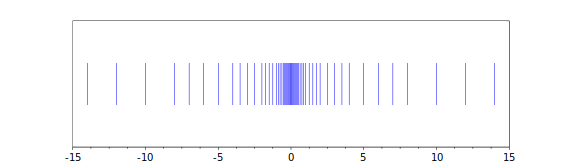
\includegraphics[width=0.9\textwidth]{toysystem_all}
\end{center}

La liste (en gras, les dénormalisés) :
-14, -12, -10, -8, -7, -6, -5, -4, -3.5, -3, -2.5, -2, -1.75, 
-1.5, -1.25, -1, -0.875, -0.75, -0.625, -0.5, -0.4375, -0.375, 
-0.3125, -0.25, \textbf{-0.1875}, \textbf{-0.125}, \textbf{-0.0625}, 
0., \textbf{0.0625}, \textbf{0.125}, \textbf{0.1875}, 0.25, 0.3125, 0.375, 
0.4375, 0.5, 0.625, 0.75, 0.875, 1, 1.25, 1.5, 1.75, 2, 2.5, 3, 
3.5, 4, 5, 6, 7, 8, 10, 12, 14.

\end{frame}

%%%%%%%%%%%%%%%%%%%%%%%%%%%%%%%%%%%%%%%%%%%%%%%%%%%%%%%%%%%%%%%%%%%%%%%%%%%%%

\begin{frame}
\frametitle{Modes d'arrondi}

Mode d'arrondi par défaut:
\begin{itemize}
\item Si $x$ est dans l'intervalle $[-\Omega,\Omega]$, on utilise RN(x) : arrondi au plus proche (round-to-nearest)
\end{itemize}

\begin{center}
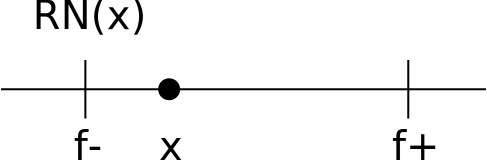
\includegraphics[width=0.4\textwidth]{roundingmodes-RN}
\end{center}

Q : connaissez-vous des réels qui ne sont pas des flottants ?

\end{frame}

%%%%%%%%%%%%%%%%%%%%%%%%%%%%%%%%%%%%%%%%%%%%%%%%%%%%%%%%%%%%%%%%%%%%%%%%%%%%%

\begin{frame}
\frametitle{Erreur d'arrondi}

On note $fl(x)$ la représentation flottante de $x$.

\begin{theorem}
(\emph{Précision machine})
Soit $x\in\RR$. 
Supposons que le système flottant est arrondir-au-plus-proche.
Si $x$ est dans l'intervalle normalisé, alors
$$
fl(x) = x(1+\delta), \qquad |\delta| \leq u= \frac{1}{2} \beta^{1-p}.
$$
où $u$ est la précision machine.
Si $x$ est dans l'intervalle dénormalisé, alors :
$$
|fl(x) - x| \leq \beta^{e_{min}-p+1}.
$$
\end{theorem}

Exercice : preuve.

En anglais : $u$ est le "unit roundoff".

Q : voyez-vous la différence entre les deux en termes d'erreur ?

\end{frame}

%%%%%%%%%%%%%%%%%%%%%%%%%%%%%%%%%%%%%%%%%%%%%%%%%%%%%%%%%%%%%%%%%%%%%%%%%%%%%

%\subsection{Les doubles IEEE}

\begin{frame}
\frametitle{Les doubles IEEE}

Les doubles IEEE 754.

\begin{center}
\begin{tabular}{|ll|}
\hline
Base $\beta$ & 2  \\
Precision $p$ & 53 \\
Exposant & 11 \\
Exposant minimum $e_{min}$ & -1022 \\
Exposant maximum $e_{max}$ & 1023 \\
Plus grand normal $\Omega$ & $\left(2-2^{-52}\right)\cdot 2^{1023} \approx 1.8\times 10^{308}$ \\
Plus petit normal $>0$ $\mu$ & $2^{-1022} \approx 2.22\times 10^{-308}$ \\
Plus petit dénormalisé $>0$ $\alpha$ & $2^{-1022-53+1} \approx 4.94\times 10^{-324}$ \\
Epsilon Machine $\epsilon_M$ & $2^{-52} \approx 2.220\times 10^{-16}$ \\
Précision machine $u$ & $2^{-53} \approx 1.110\times 10^{-16}$ \\
\hline
\end{tabular}
\end{center}

\end{frame}

%%%%%%%%%%%%%%%%%%%%%%%%%%%%%%%%%%%%%%%%%%%%%%%%%%%%%%%%%%%%%%%%%%%%%%%%%%%%%

\begin{frame}[containsverbatim]
\frametitle{Les doubles IEEE}

Les doubles positifs, avec une échelle "artistique".

\begin{center}
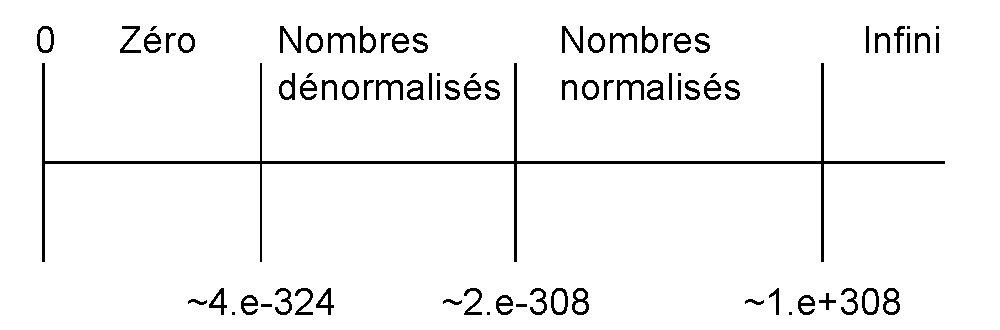
\includegraphics[width=0.9\textwidth]{subnormal-numbers.pdf}
\end{center}

\end{frame}

%%%%%%%%%%%%%%%%%%%%%%%%%%%%%%%%%%%%%%%%%%%%%%%%%%%%%%%%%%%%%%%%%%%%%%%%%%%%%
\section{Erreur}

%%%%%%%%%%%%%%%%%%%%%%%%%%%%%%%%%%%%%%%%%%%%%%%%%%%%%%%%%%%%%%%%%%%%%%%%%%%%%
\begin{frame}
\frametitle{Erreur}
  \begin{columns}
    \column{0.5\textwidth}
    
    \column{0.5\textwidth}
    {\usebeamercolor[fg]{title}\huge{Erreur}}
	
	Comment calculer une erreur absolue, relative, le 
	nombre de chiffres significatifs, l'erreur forward/backward 
	et le conditionnement.
  \end{columns}
\end{frame}

%%%%%%%%%%%%%%%%%%%%%%%%%%%%%%%%%%%%%%%%%%%%%%%%%%%%%%%%%%%%%%%%%%%%%%%%%%%%%

\begin{frame}
\frametitle{Erreur relative, absolue}

% Source : Accuracy and stability of numerical algorithms.

\begin{definition}
(\emph{Erreur absolue, relative})
Soit:
\begin{itemize}
\item un nombre réel : $x$,
\item son approximation : $\hat{x}$.
\end{itemize}
Alors, l'erreur absolue est:
$$
E_{abs}(x,\hat{x}) = |x-\hat{x}|
$$
et l'erreur relative est :
$$
E_{rel}(x,\hat{x}) = \frac{|x-\hat{x}|}{|x|}
$$
si $x\neq 0$.
\end{definition}

\end{frame}

%%%%%%%%%%%%%%%%%%%%%%%%%%%%%%%%%%%%%%%%%%%%%%%%%%%%%%%%%%%%%%%%%%%%%%%%%%%%%

\def\blueA{\textcolor{blue}{A}}
\def\redB{\textcolor{red}{B}}
\def\dgrenC{\textcolor{darkgreen}{C}}
\def\violetD{\textcolor{violet}{D}}

\begin{frame}
\frametitle{Erreur relative, absolue}

% Source : Accuracy and stability of numerical algorithms.

\begin{example}

\begin{footnotesize}
\begin{center}
\begin{tabular}{lllll}
& $x$ & $\hat{x}$ & $E_{abs}$ & $E_{rel}$ \\
\hline
\blueA & 1. & 2. & 1. & 1. \\
\redB & 1. & 1.000001 & 9.99999999918e-07& 9.99999999918e-07\\
\dgrenC & 1.e100 & 1.000001e100 & 9.99999999909e+93 & 9.99999999909e-07 \\
\violetD & 0. & 1.e-100 & 1e-100 & inf
\end{tabular}
\end{center}
\end{footnotesize}

Question - Analyse:

\begin{tabular}{l|l|l}
& Relative & Absolue \\
\hline
Grande & ?  & ? \\
Petite & ? & ?
\end{tabular}

\end{example}

\end{frame}
%%%%%%%%%%%%%%%%%%%%%%%%%%%%%%%%%%%%%%%%%%%%%%%%%%%%%%%%%%%%%%%%%%%%%%%%%%%%%

\begin{frame}
\frametitle{Erreur relative, absolue}

% Source : Accuracy and stability of numerical algorithms.

\begin{example}

\begin{footnotesize}
\begin{center}
\begin{tabular}{lllll}
& $x$ & $\hat{x}$ & $E_{abs}$ & $E_{rel}$ \\
\hline
\blueA & 1. & 2. & 1. & 1. \\
\redB & 1. & 1.000001 & 9.99999999918e-07& 9.99999999918e-07\\
\dgrenC & 1.e100 & 1.000001e100 & 9.99999999909e+93 & 9.99999999909e-07 \\
\violetD & 0. & 1.e-100 & 1e-100 & inf
\end{tabular}
\end{center}
\end{footnotesize}

Analyse:

\begin{tabular}{l|l|l}
& Relative & Absolue \\
\hline
Grande & \blueA, \violetD & \blueA, \dgrenC \\
Petite & \redB, \dgrenC & \redB, \violetD
\end{tabular}

\end{example}

\end{frame}



%%%%%%%%%%%%%%%%%%%%%%%%%%%%%%%%%%%%%%%%%%%%%%%%%%%%%%%%%%%%%%%%%%%%%%%%%%%%%

\begin{frame}
\frametitle{Erreur relative, absolue}

En général:
\begin{itemize}
\item Si $x\neq 0$, utiliser l'erreur relative.
\item Si $x= 0$, utiliser l'erreur absolue.
\end{itemize}

Si $\bx\in\RR^n$ est un vecteur, on peut utiliser l'erreur relative 
composante-par-composante:
$$
\max_{i=1,...,n} \left| \frac{x_i-\hat{x}_i}{x_i} \right|
$$

\end{frame}

%%%%%%%%%%%%%%%%%%%%%%%%%%%%%%%%%%%%%%%%%%%%%%%%%%%%%%%%%%%%%%%%%%%%%%%%%%%%%

\begin{frame}
\frametitle{Nombre de chiffres corrects}

\begin{definition}
(\emph{Nombre de chiffres corrects en base $\beta$ - la log-erreur relative})
La Log-Erreur relative en base $\beta$ est définie par :
$$
LRE_\beta(x,\hat{x})
=-\log_{\beta}(E_{rel}(x,\hat{x}))
$$
\end{definition}

Avec des doubles:

\begin{center}
\begin{tabular}{l|ll}
        & $\beta=2$ & $\beta=10$ \\
\hline
LRE min & 0     & 0      \\
LRE max & 53    & 15.95
\end{tabular}
\end{center}

\end{frame}

%%%%%%%%%%%%%%%%%%%%%%%%%%%%%%%%%%%%%%%%%%%%%%%%%%%%%%%%%%%%%%%%%%%%%%%%%%%%%

\begin{frame}
\frametitle{Précision : exemples de tests}

Calcul : distributions.

Données de référence : Mathematica 5.2, ELV (Knüsel, 2003).

\begin{center}
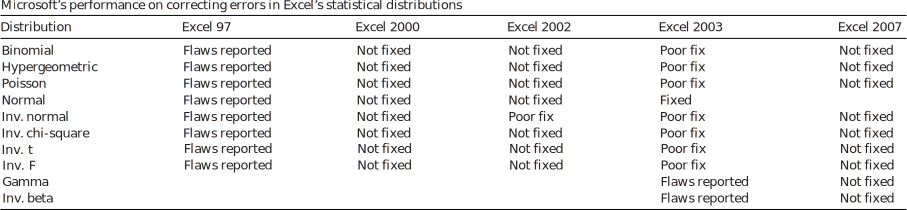
\includegraphics[width=0.8\textwidth]{Yalta-2008-excel}
\end{center}

\begin{center}
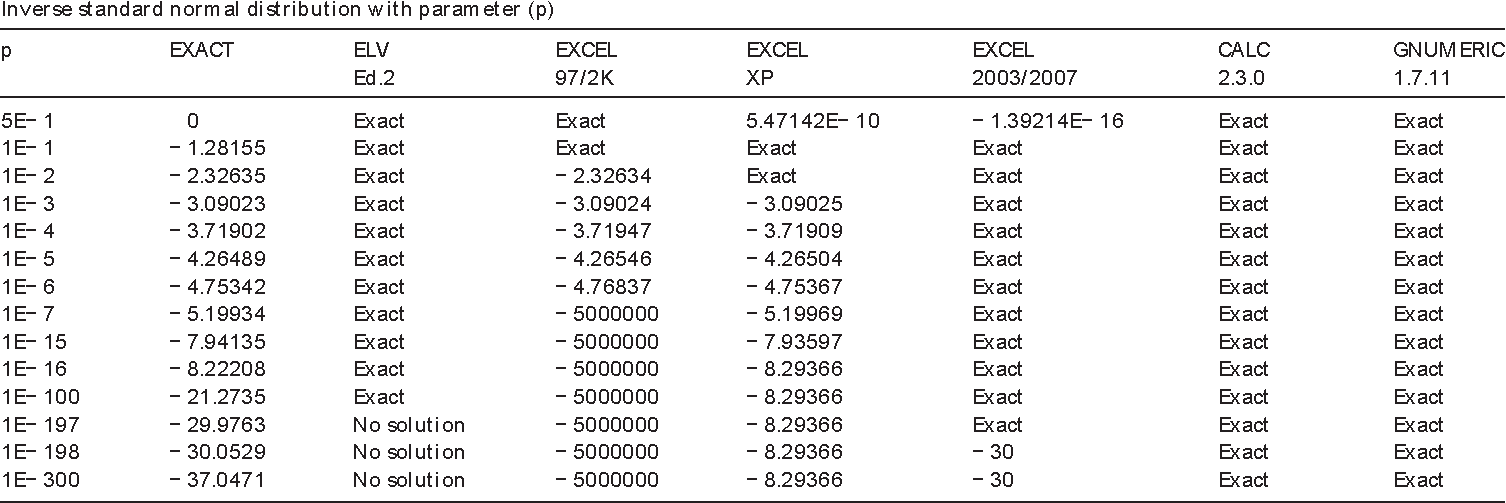
\includegraphics[width=0.8\textwidth]{Yalta-2008-invnorm}
\end{center}

Ref. : Yalta (2008)

\end{frame}

%%%%%%%%%%%%%%%%%%%%%%%%%%%%%%%%%%%%%%%%%%%%%%%%%%%%%%%%%%%%%%%%%%%%%%%%%%%%%

\begin{frame}
\frametitle{Précision : exemples de tests}

Calcul : régression linéaire.

Données de référence : (American) National Institute of Standards and Technology (NIST), 
Statistical Reference Data sets (StRD).

\begin{center}
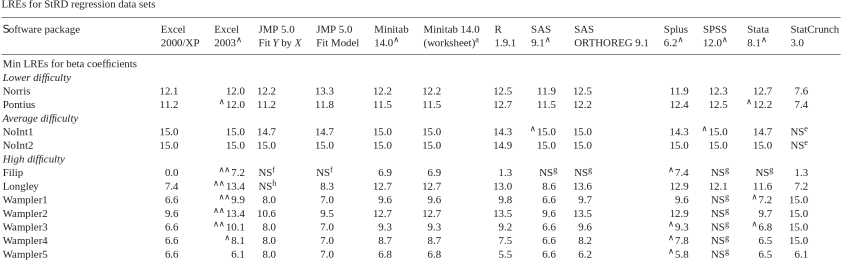
\includegraphics[width=1.\textwidth]{Keeling-Pavur-2007}
\end{center}

Ref. : extrait de Keelinga, Pavurb (2007) (le tableau original 
contenait d'autres comparaisons).

\end{frame}


%%%%%%%%%%%%%%%%%%%%%%%%%%%%%%%%%%%%%%%%%%%%%%%%%%%%%%%%%%%%%%%%%%%%%%%%%%%%%

\begin{frame}
\frametitle{Erreur forward, backward}

\begin{itemize}
\item On considère une fonction $G$, un réel d'entrée $x$ et 
on veut calculer 
$$
y=G(x).
$$
\item Soit $\hat{y}$ une approximation de $y$ :
$$
\hat{y} \approx G(x)
$$
\item Comment mesurer la "qualité" de $\hat{y}$ ?
\end{itemize}

\end{frame}

%%%%%%%%%%%%%%%%%%%%%%%%%%%%%%%%%%%%%%%%%%%%%%%%%%%%%%%%%%%%%%%%%%%%%%%%%%%%%

\begin{frame}
\frametitle{Erreur forward, backward}

Mesure possible : l'erreur est faible si 
$$
E_{rel}(y,\hat{y}) = \frac{|y-\hat{y}|}{|y|} \approx u
$$

Autre mesure : pour quelle donnée d'entrée avons nous résolu le problème ?

\emph{"Quelle perturbation de l'entrée $x$ est nécessaire 
pour obtenir exactement $\hat{y}$ ?}

Pour quelle valeur de $\Delta x$ avons-nous:
$$
\hat{y}=G(x+\Delta x)
$$

Si il y a plusieurs $\Delta x$, on prend le plus petit. 
\end{frame}

%%%%%%%%%%%%%%%%%%%%%%%%%%%%%%%%%%%%%%%%%%%%%%%%%%%%%%%%%%%%%%%%%%%%%%%%%%%%%

\begin{frame}
\frametitle{Erreur forward, backward}

Deux types d'erreur:
\begin{itemize}
\item Erreur forward : $E_{rel}(y,\hat{y})$ ou $E_{abs}(y,\hat{y})$
\item Erreur backward : $|\Delta x|/|x|$ (relative) ou $|\Delta x|$ (absolue)
\end{itemize}

Erreurs forward et backward pour $y=G(x)$. 

Solide : exact. Pointillé : calculé.

\begin{center}
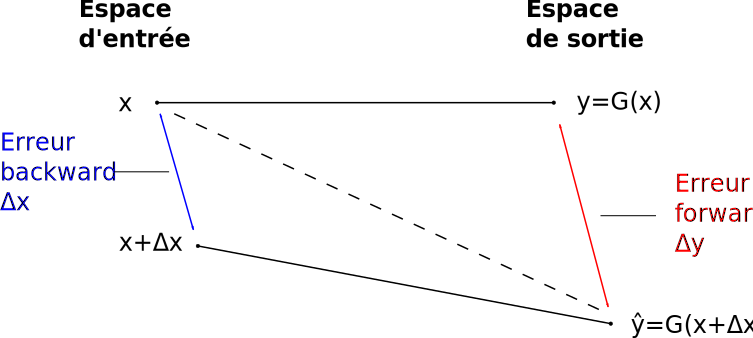
\includegraphics[width=0.8\textwidth]{forwardbackward}
\end{center}

\end{frame}

%%%%%%%%%%%%%%%%%%%%%%%%%%%%%%%%%%%%%%%%%%%%%%%%%%%%%%%%%%%%%%%%%%%%%%%%%%%%%

\begin{frame}
\frametitle{Conditionnement}

\begin{definition}
(\emph{Conditionnement dans $\RR$})
Soit $G$ une fonction continûment dérivable telle que 
$G^{\prime\prime}$ est bornée. 
On suppose que $G(x)$ n'est pas nul. 
Le conditionnement de $G$ est :
$$
K_G(x)= \lim_{\Delta x \rightarrow 0} \left| \frac{E_{rel}(y,\hat{y})}{E_{rel}(x,\hat{x})}\right|
$$
avec
$$
\hat{x}=x+\Delta x, \qquad y=G(x) \textrm{ et }
\hat{y} = G(x+\Delta x).
$$
\end{definition}

\emph{Le coefficient multiplicatif $K_G$ mesure le rapport entre 
l'erreur relative sur $y$ et l'erreur relative sur $x$.}

\end{frame}

%%%%%%%%%%%%%%%%%%%%%%%%%%%%%%%%%%%%%%%%%%%%%%%%%%%%%%%%%%%%%%%%%%%%%%%%%%%%%

\begin{frame}
\frametitle{Conditionnement}

Quand $\Delta x$ est petit, on a 
$$
E_{rel}(y,\hat{y}) \approx K_G(x) \times E_{rel}(x,\hat{x})
$$
donc :
$$
LRE_{10}(y,\hat{y})
\approx LRE_{10}(x,\hat{x}) - \log_{10}(K_G(x)).
$$

Conclusion : $\log_{10}(K_G(x))$ est le nombre 
de chiffres décimaux perdus dans $y$ par rapport à $x$ à cause du 
conditionnement dans $G$.

\begin{theorem}
(\emph{Conditionnement dans $\RR$})
Sous les mêmes conditions, le conditionnement de $G$ est :
$$
K_G(x)=\left| \frac{x G^\prime(x)}{G(x)}\right|.
$$
\end{theorem}

\end{frame}

%%%%%%%%%%%%%%%%%%%%%%%%%%%%%%%%%%%%%%%%%%%%%%%%%%%%%%%%%%%%%%%%%%%%%%%%%%%%%

\begin{frame}
\frametitle{Conditionnement}

Règle générale:
$$
\textrm{erreur forward } \lesssim \textrm{ conditionnement } \times  
\textrm{ erreur backward } 
$$

Donc:
$$
\textrm{ erreur backward petite } \Rightarrow \textrm{ erreur forward petite}
$$
mais pas le contraire.
\end{frame}

%%%%%%%%%%%%%%%%%%%%%%%%%%%%%%%%%%%%%%%%%%%%%%%%%%%%%%%%%%%%%%%%%%%%%%%%%%%%%

\begin{frame}
\frametitle{Conditionnement : exemple de log1p}

\begin{example}

$$
G(x)=\log(x)
$$
Le conditionnement est:
$$
K_{\log}(x)=\left|\frac{1}{\log(x)}\right|,
$$
qui est grand pour $x\approx 1$ car $\log(1)=0$. 

Or $\log(1+\Delta x) \approx 0$, lorsque $\Delta x$ est petit. 

Donc un petit changement autour de $x=1$ provoque sur $\log(x)$ :
\begin{itemize}
\item un petit changement absolu
\item un grand changement relatif
\end{itemize}

Le rôle de la fonction $\textrm{log1p}(x)=\log(1+x)$ est 
de résoudre ce problème de précision.
\end{example}

\end{frame}


%%%%%%%%%%%%%%%%%%%%%%%%%%%%%%%%%%%%%%%%%%%%%%%%%%%%%%%%%%%%%%%%%%%%%%%%%%%%%

\begin{frame}[containsverbatim]
\frametitle{Conditionnement : exemple de log1p}

Application de log1p pour les probabilités.

Calcul de la fonction de répartition inverse (quantile) de la 
loi exponentielle de moyenne $\mu$.

La fonction de répartition est :
$$
p=F(x) = 1-e^{-\frac{x}{\mu}}
$$
La fonction de répartition inverse est :
$$
x = F^{-1}(p)=-\mu\log(1-p)
$$

\end{frame}
%%%%%%%%%%%%%%%%%%%%%%%%%%%%%%%%%%%%%%%%%%%%%%%%%%%%%%%%%%%%%%%%%%%%%%%%%%%%%

\begin{frame}[containsverbatim]
\frametitle{Conditionnement : exemple de log1p}

Calcul de $F^{-1}(p)$ : pour $\mu=1$ et $p=10^{-20}$, le quantile exact est $x=10^{-20}$. 

  \begin{columns}
    \column{0.5\textwidth}
Naïf :
\begin{lstlisting}
def expinv(p,mu):
    if p==1.0:
        x=float("inf")
    else:
        x=-mu*log(1.0-p)
    return x

>>> expinv(1.e-20,1.0)
-0.0
\end{lstlisting}

    \column{0.5\textwidth}

Robuste :
\begin{lstlisting}
def expinvMieux(p,mu):
    if p==1.0:
        x=float("inf")
    else:
        x=-mu*log1p(-p)
    return x

>>> expinvMieux(1.e-20,1.0) 
1e-20
\end{lstlisting}

  \end{columns}

\end{frame}
%%%%%%%%%%%%%%%%%%%%%%%%%%%%%%%%%%%%%%%%%%%%%%%%%%%%%%%%%%%%%%%%%%%%%%%%%%%%%

\begin{frame}[containsverbatim]
\frametitle{Conditionnement : exemple de log1p}

  \begin{columns}
    \column{0.4\textwidth}

"Mais je ne traite pas des probabilité aussi faibles !" 

Certes, il reste que pour des probabilités décroissantes ($10^{-1}$, 
$10^{-2}$, $10^{-3}$, etc...),
il y a une perte progressive des chiffres corrects.

Calcul de $F(x)$ : utiliser \textrm{expm1} (sinon cancellation).

    \column{0.6\textwidth}

\begin{center}
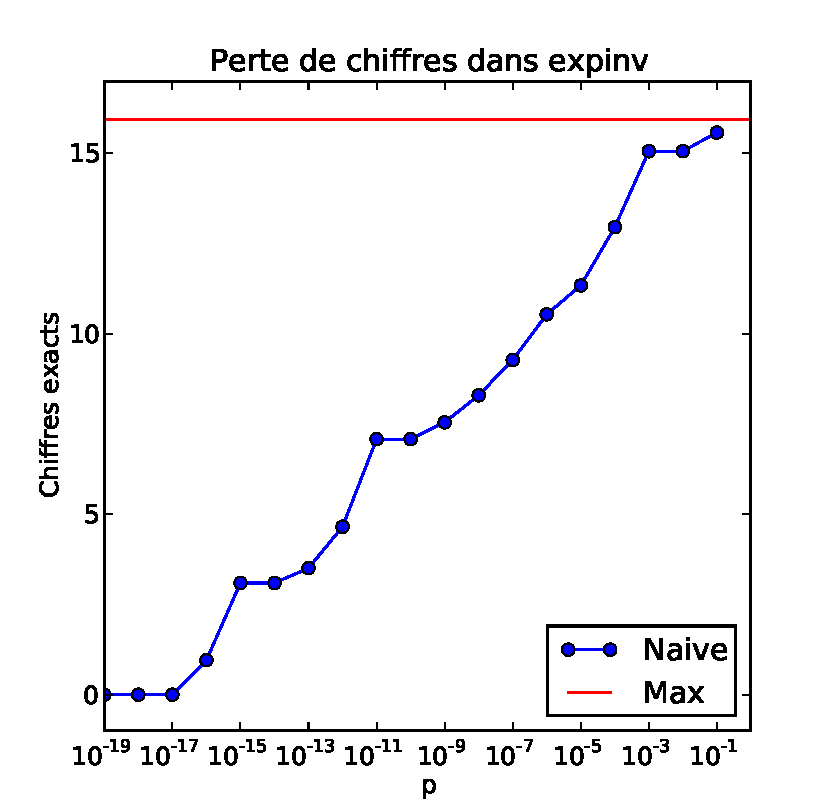
\includegraphics[width=1.0\textwidth]{expinv-perte}
\end{center}

  \end{columns}

\end{frame}

%%%%%%%%%%%%%%%%%%%%%%%%%%%%%%%%%%%%%%%%%%%%%%%%%%%%%%%%%%%%%%%%%%%%%%%%%%%%%

\begin{frame}[containsverbatim]
\frametitle{Conditionnement : quantiles loi normale}

La fonction \textrm{norminv} (quantile de la loi normale) 
est mal conditionnée en $p=0.5$ et $p=1$.

\begin{center}
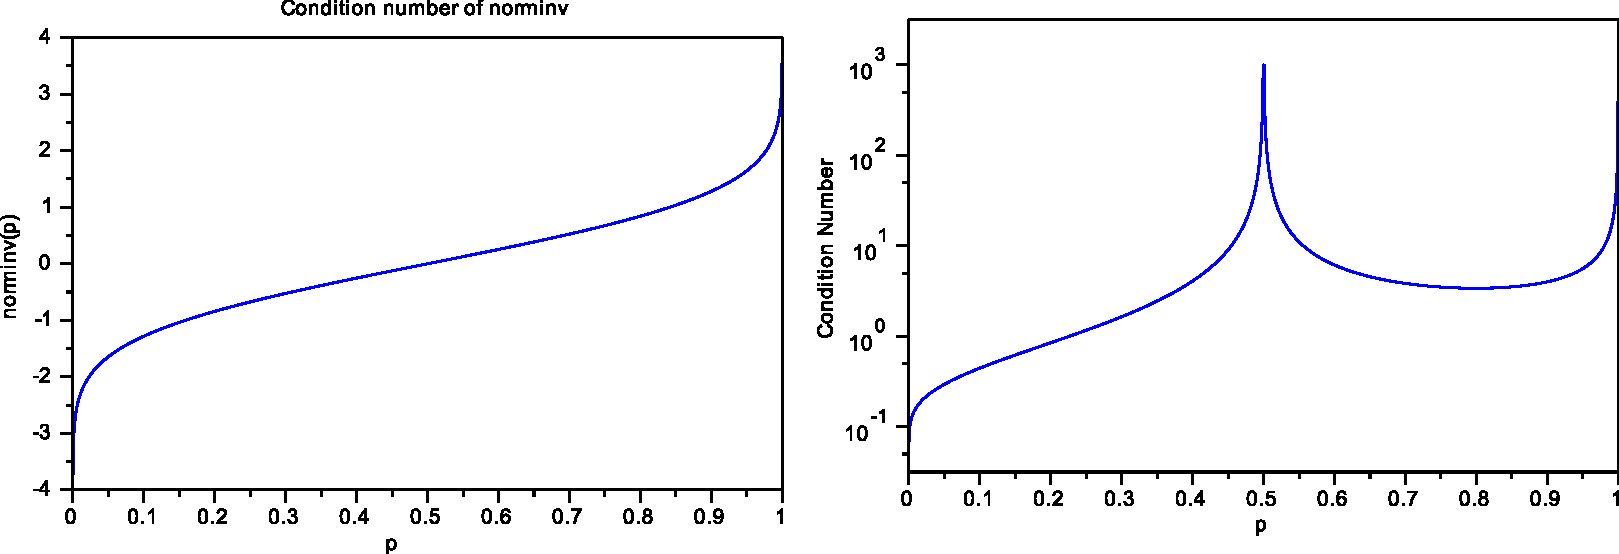
\includegraphics[width=\textwidth]{condnorminv2}
\end{center}

Ref. Edelman (2010)

\end{frame}

%%%%%%%%%%%%%%%%%%%%%%%%%%%%%%%%%%%%%%%%%%%%%%%%%%%%%%%%%%%%%%%%%%%%%%%%%%%%%

\section{Tests}

%%%%%%%%%%%%%%%%%%%%%%%%%%%%%%%%%%%%%%%%%%%%%%%%%%%%%%%%%%%%%%%%%%%%%%%%%%%%%
\begin{frame}
\frametitle{Tests}
  \begin{columns}
    \column{0.5\textwidth}
    
    \column{0.5\textwidth}
    {\usebeamercolor[fg]{title}\huge{Tests}}
	
	Utiliser une librairie d'assertions. 
	Comment tester un calcul probabiliste ?
  \end{columns}
\end{frame}

%%%%%%%%%%%%%%%%%%%%%%%%%%%%%%%%%%%%%%%%%%%%%%%%%%%%%%%%%%%%%%%%%%%%%%%%%%%%%
\begin{frame}
\frametitle{Assertions : pourquoi ?}

Pourquoi utiliser une librairie d'assertions ?
\begin{itemize}
\item Pour tester le comportement d'une fonction. 
\item Pour structurer les tests unitaires. 
\item Faciliter le test de calculs numériques, en particulier, 
issus d'algorithmes de calcul (par exemple itératifs)
\item Préciser la notion de valeurs numériques "presque égales", 
c'est à dire telles que l'erreur relative est "petite".
\end{itemize}

\end{frame}

%%%%%%%%%%%%%%%%%%%%%%%%%%%%%%%%%%%%%%%%%%%%%%%%%%%%%%%%%%%%%%%%%%%%%%%%%%%%%
\begin{frame}[containsverbatim]
\frametitle{Démarrage}

Comme exemple, nous considérons les fonctions \sciobj{assert} de Scilab. 

Mais tous les languages ont implémenté le même concept :
\begin{itemize}
\item Matlab : Eddins (2009)
\item C++ : Cppunit
\item Java : Junit
\item Python : PyUnit
\item Fortran : Flibs/ftnunit (Sourceforge)
\end{itemize}

\end{frame}

% %%%%%%%%%%%%%%%%%%%%%%%%%%%%%%%%%%%%%%%%%%%%%%%%%%%%%%%%%%%%%%%%%%%%%%%%%%%%%
% \begin{frame}
% \frametitle{Anecdotes et historique}

% En ce qui me concerne, voici un historique bref.

% \begin{itemize}
% \item En 2000-2003, mon épouse travaille pour Philips, 
% en prestation sur la création de tests pour un décodeur numérique. 
% En 2003, le projet de 80 ingénieurs est fermé : le décodeur ne respecte pas le 
% standard, mais une société de 4 ingénieurs en 
% Roumanie a développé un meilleur produit en 2 ans (rachetée par Philips). 
% Ils utilisaient des tests unitaires depuis le début...
% \item En 2001-2003, j'applique ces idées au code de ma thèse. 
% \item En 2004-2006, Didier Poizat et moi-même créons une 
% librairie d'assertions pour un code Fortran 77 à l'IFP. 
% \item En 2005-2007, je porte une adaptation de ce code en 
% Fortran 90 avec Arjen Markus pour Flibs (Sourceforge).
% \item En 2007-2011, j'adapte ces concepts à Scilab.
% \end{itemize}

% \end{frame}

%%%%%%%%%%%%%%%%%%%%%%%%%%%%%%%%%%%%%%%%%%%%%%%%%%%%%%%%%%%%%%%%%%%%%%%%%%%%%
\begin{frame}[containsverbatim]
\frametitle{L'idée principale : \sciobj{assert\_checktrue}}

Exemple dans Scilab : les fonctions \sciobj{assert}.

La fonction \sciobj{assert\_checktrue} vérifie qu'une matrice de booléens 
est vraie. 
On suppose que la fonction \sciobj{G} prend un réel et renvoit un booléen.

\begin{lstlisting}
x=2
computed=G(x)
assert_checktrue ( computed )
\end{lstlisting}

Deux cas :
\begin{enumerate}
\item Si (au moins) une des entrées est fausse, une erreur est générée : 
le code s'arrête.
\item Sinon, la fonction ne fait rien.
\end{enumerate}

\end{frame}

%%%%%%%%%%%%%%%%%%%%%%%%%%%%%%%%%%%%%%%%%%%%%%%%%%%%%%%%%%%%%%%%%%%%%%%%%%%%%
\begin{frame}[containsverbatim]
\frametitle{L'idée principale : \sciobj{assert\_checkequal}}

La fonction \sciobj{assert\_checkequal} vérifie que deux valeurs sont égales. 
\begin{lstlisting}
x=2
computed=G(x)
expected=3
assert_checkequal ( computed , expected )
\end{lstlisting}

Deux cas :
\begin{enumerate}
\item Si les deux valeurs ne sont pas égales, une erreur est générée : 
le code s'arrête.
\item Sinon, la fonction ne fait rien.
\end{enumerate}

\end{frame}

%%%%%%%%%%%%%%%%%%%%%%%%%%%%%%%%%%%%%%%%%%%%%%%%%%%%%%%%%%%%%%%%%%%%%%%%%%%%%
\begin{frame}[containsverbatim]
\frametitle{L'idée principale : \sciobj{assert\_checkalmostequal}}

La fonction \sciobj{assert\_checkalmostequal} vérifie qu'une 
valeur calculée est proche d'une valeur attendue. 

Dans l'exemple suivant, on vérifie que 1.23456 est proche de 
1.23457 avec une erreur relative de $10^{-4}$ :
\begin{lstlisting}
assert_checkalmostequal ( 1.23456 , 1.23457 , 1.e-4 )
\end{lstlisting}

\end{frame}

%%%%%%%%%%%%%%%%%%%%%%%%%%%%%%%%%%%%%%%%%%%%%%%%%%%%%%%%%%%%%%%%%%%%%%%%%%%%%
\begin{frame}[containsverbatim]
\frametitle{\sciobj{test\_run}}

\begin{lstlisting}
-->test_run("development_tools|assert")
TMPDIR = C:\Users\C61372\AppData\Local\Temp\SCI_TMP_4924_
01/01-[development_tools|assert] : 
01/11-[development_tools|assert] checkalmostequal..passed
02/11-[development_tools|assert] checkequal........passed
03/11-[development_tools|assert] checkerror........passed
04/11-[development_tools|assert] checkfalse........passed
05/11-[development_tools|assert] checkfilesequal...passed
06/11-[development_tools|assert] checktrue.........passed
07/11-[development_tools|assert] comparecomplex....passed
08/11-[development_tools|assert] computedigits.....passed
09/11-[development_tools|assert] cond2reltol.......passed
10/11-[development_tools|assert] cond2reqdigits....passed
11/11-[development_tools|assert] generror..........passed
---------------------------------------------------------
Summary
tests             11 - 100 %
passed            11 - 100 %
failed             0 -   0 %
skipped            0
length             43.95 sec
----------------------------------------------------------
\end{lstlisting}

\end{frame}

%%%%%%%%%%%%%%%%%%%%%%%%%%%%%%%%%%%%%%%%%%%%%%%%%%%%%%%%%%%%%%%%%%%%%%%%%%%%%
\begin{frame}[containsverbatim]
\frametitle{Focus sur \sciobj{assert\_checkalmostequal}}

Séquences d'appel possibles :
\begin{lstlisting}
assert_checkalmostequal(computed,expected)
assert_checkalmostequal(computed,expected,reltol)
assert_checkalmostequal(computed,expected,reltol,abstol)
assert_checkalmostequal(computed,expected,reltol,abstol,..
    comptype)
\end{lstlisting}
où
\begin{itemize}
\item \sciobj{reltol} : l'erreur relative (défaut : $\sqrt{\epsilon_M}$)
\item \sciobj{abstol} : l'erreur relative (défaut : 0)
\item \sciobj{comptype} : type de norme pour la comparaison. 
Pour une norme matricielle : "matrix", pour une 
comparaison élément-par-élément : "element" (défaut : "element")
\end{itemize}

\end{frame}

%%%%%%%%%%%%%%%%%%%%%%%%%%%%%%%%%%%%%%%%%%%%%%%%%%%%%%%%%%%%%%%%%%%%%%%%%%%%%
\begin{frame}[containsverbatim]
\frametitle{Ajuster la tolérance}

Comment tenir compte du conditionnement pour ajuster la tolérance 
lors du test d'une fonction élémentaire ?

Le conditionnement de $G$ est :
$$
K_G(x)
=\lim_{\Delta x \rightarrow 0} \left| \frac{E_{rel}(y,\hat{y})}{E_{rel}(x,\hat{x})}\right|
 = \left| \frac{x G^\prime(x)}{G(x)}\right|.
$$
avec
$$
\hat{x}=x+\Delta x, \qquad y=G(x) \textrm{ et }
\hat{y} = G(x+\Delta x).
$$
Souhaite donc :
$$
|G(x+\Delta x)-G(x)| \approx K_G(x) \frac{|\Delta x|}{|x|} |G(x)|
$$
où $\Delta x$ est la distance entre $x$ et son flottant le plus proche.

Ref.: Brorson, Edelman, Moskowitz, 2012
\end{frame}

%%%%%%%%%%%%%%%%%%%%%%%%%%%%%%%%%%%%%%%%%%%%%%%%%%%%%%%%%%%%%%%%%%%%%%%%%%%%%
\begin{frame}[containsverbatim]
\frametitle{Ajuster la tolérance}

Or, on peut démontrer que, pour deux flottants $x$ et $y$ voisins, 
on a :
$$
|x-y|\leq \epsilon_M |x|
$$
où $y=x^+$ ou bien $y=x^-$ et 
$$
\epsilon=2^{1-p}=2^{-52}\approx 2.220\times 10^{-16},
$$
si on utilise des doubles. 

Cela implique 
$$
\frac{|\Delta x|}{|x|} \leq \epsilon_M.
$$

\end{frame}

%%%%%%%%%%%%%%%%%%%%%%%%%%%%%%%%%%%%%%%%%%%%%%%%%%%%%%%%%%%%%%%%%%%%%%%%%%%%%
\begin{frame}[containsverbatim]
\frametitle{Ajuster la tolérance}
On demande donc :
$$
\frac{|G_{calcul}-G_{exact}|}{|G_{exact}|} \leq C K_G(x) \epsilon_M 
$$
où $C$ est une petite constante. 

Si 
$$
G_{exact} \neq 0,
$$
on peut donc utiliser l'erreur relative :
$$
reltol = C K_G(x) \epsilon_M.
$$


Sauf si il s'agit d'une fausse singularité de $K_G(x)$, si 
$$
G_{exact} = 0,
$$
alors l'erreur absolue :
$$
abstol = C K_G(x) \epsilon_M |G_{exact}| = 0
$$
ne peut pas être utilisée.

\end{frame}

%%%%%%%%%%%%%%%%%%%%%%%%%%%%%%%%%%%%%%%%%%%%%%%%%%%%%%%%%%%%%%%%%%%%%%%%%%%%%
\begin{frame}[containsverbatim]
\frametitle{Ajuster la tolérance}

Ajuster $C$ :
\begin{itemize}
\item Augmenter $C$ augmente la tolérance : $C$ doit être 
le plus petit possible. 

\item En pratique, commencer par $C=0$ car certaines fonctions 
sont telles que, si $x$ est un flottant, alors $G_{calcul}$ est le 
flottant le plus proche de la valeur exacte $G(x)$. Par exemple : 
$+,-,*,/$ et $\sqrt{x}$.

\item Puis, prendre $C=1,2,3,...$ dans cet ordre 
jusqu'à faire passer tous les tests.

\item Etre obligé de prendre $C\geq 10$ signale une implémentation sous-optimale.
\end{itemize}
\end{frame}

%%%%%%%%%%%%%%%%%%%%%%%%%%%%%%%%%%%%%%%%%%%%%%%%%%%%%%%%%%%%%%%%%%%%%%%%%%%%%
\begin{frame}[containsverbatim]
\frametitle{Tester un calcul probabiliste}

Difficulté : nous travaillons sur des calculs probabilistes, 
et non pas sur des calculs déterministes.

Hypothèse :
$$
Y=G(X)
$$
avec $X$ une variable aléatoire. 

Conséquence : $Y$ est une variable aléatoire que l'on souhaite tester.
\end{frame}

%%%%%%%%%%%%%%%%%%%%%%%%%%%%%%%%%%%%%%%%%%%%%%%%%%%%%%%%%%%%%%%%%%%%%%%%%%%%%
\begin{frame}[containsverbatim]
\frametitle{Tester un calcul probabiliste}

D'abord, on devrait utiliser des algorithmes de qualité :
\begin{itemize}
\item un générateur de nombres pseudo-aléatoires 
uniformes de qualité,
\item des algorithmes de générations de nombres non uniformes 
de qualité,
\item des algorithmes de calcul de fonctions de distribution 
de qualité,
\item des techniques de résolution de systèmes linéaires 
 de qualité (par exemple, pivot de Gauss avec permutation des lignes 
utilisant l'interface LAPACK),
\item etc...
\end{itemize}

Quel sens a une validation, si on sait par avance que les algorithmes 
utilisés sont mauvais ?

\end{frame}

%%%%%%%%%%%%%%%%%%%%%%%%%%%%%%%%%%%%%%%%%%%%%%%%%%%%%%%%%%%%%%%%%%%%%%%%%%%%%

\begin{frame}
\frametitle{Tester un calcul probabiliste}
Générateurs Pseudo-Aléatoires Uniformes
\begin{itemize}
\item Dans la fonction \pyobj{rand()} du language C.
\item Dans la fonction \pyobj{grand} de Scilab : URAND
    \begin{itemize}
    \item Type de générateur : linéaire congruentiel.
	\item Auteurs : M. Malcolm, C. Moler (1973).
	\item Période : $2^{31}\approx 2.1\times 10^9$
    \end{itemize}  
\item Dans la fonction \pyobj{grand} 
de Scilab : Mersenne-Twister (par défaut)
    \begin{itemize}
    \item Type de générateur : Linear Feedback Shift Register.
    \item Code : MT19937 par M. Matsumoto, T. Nishimura (1998).
    \item Période : $2^{19937}\approx 10^{6001}$.
    \end{itemize}
\end{itemize}
\end{frame}

%%%%%%%%%%%%%%%%%%%%%%%%%%%%%%%%%%%%%%%%%%%%%%%%%%%%%%%%%%%%%%%%%%%%%%%%%%%%%
\begin{frame}[containsverbatim]
\frametitle{Tester un calcul probabiliste}

Exemple : 
Je génère $400\times 10^7$ nombres uniformes pseudo-aléatoires 
dans le carré unité en dimension 2, puis je ne garde 
que les nombres dans l'intervalle $[0,t]^2$, avec $t=0.001$ 
(nécessite $\approx$ 15 min). 

\end{frame}

%%%%%%%%%%%%%%%%%%%%%%%%%%%%%%%%%%%%%%%%%%%%%%%%%%%%%%%%%%%%%%%%%%%%%%%%%%%%%
\begin{frame}[containsverbatim]
\frametitle{Tester un calcul probabiliste}

\begin{center}
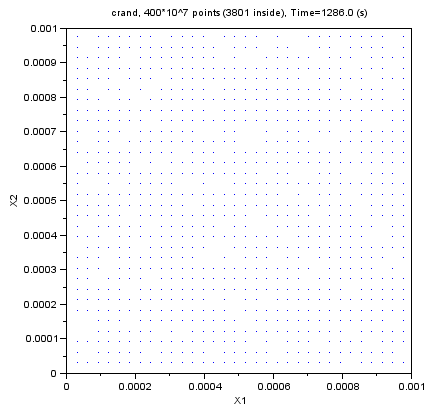
\includegraphics[width=0.3\textwidth]{crand}
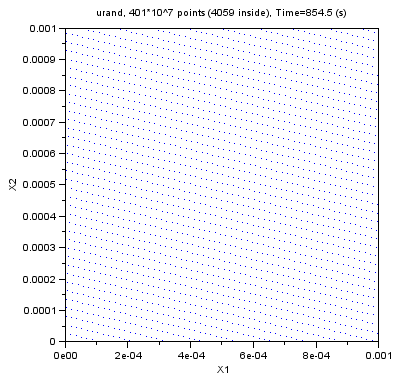
\includegraphics[width=0.3\textwidth]{grand-urand}
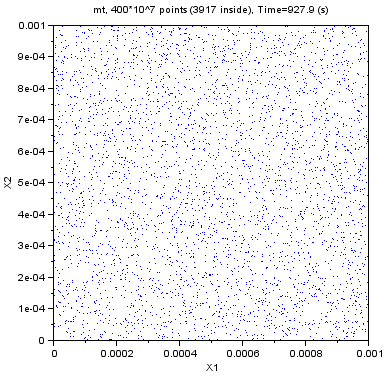
\includegraphics[width=0.3\textwidth]{grand-mt}
\end{center}

Moralité : dans Scilab, le statisticien n'utilise pas \pyobj{rand}, mais il utilise 
\pyobj{grand}.

\end{frame}
%%%%%%%%%%%%%%%%%%%%%%%%%%%%%%%%%%%%%%%%%%%%%%%%%%%%%%%%%%%%%%%%%%%%%%%%%%%%%
\begin{frame}[containsverbatim]
\frametitle{Tester un calcul probabiliste}

Exemple : estimer une moyenne empirique avec 
$$
M_n = \frac{1}{n} \sum_{i=1}^n y_i
$$
où 
$$
y_i = G(x_i), \quad i=1,2,\ldots,n,
$$
et $X$ suit une distribution donnée.

Comment tester le résultat ?

\end{frame}

%%%%%%%%%%%%%%%%%%%%%%%%%%%%%%%%%%%%%%%%%%%%%%%%%%%%%%%%%%%%%%%%%%%%%%%%%%%%%
\begin{frame}[containsverbatim]
\frametitle{Tester un calcul probabiliste}

Test :
\begin{lstlisting}
// 1000 valeurs U(0,1) :
x=grand(1000,1,"unf",0,1)
y=G(x)
computed=mean(y)
expected=0.5
reltol = TODO // <- ?
assert_checkalmostequal(computed,expected,reltol)
\end{lstlisting}

Questions :
\begin{itemize}
\item Comment déterminer \sciobj{expected} ?
\item Comment déterminer \sciobj{reltol} ?
\item Dois-je prendre une erreur absolue ou relative ?
\item Et si je relance une simulation ?
\item Quelle erreur dûe au conditionnement ?
\item Quelle erreur dûe à l'estimateur ?
\end{itemize}

\end{frame}

%%%%%%%%%%%%%%%%%%%%%%%%%%%%%%%%%%%%%%%%%%%%%%%%%%%%%%%%%%%%%%%%%%%%%%%%%%%%%
\begin{frame}[containsverbatim]
\frametitle{Comment déterminer \sciobj{expected} ?}

\begin{enumerate}
\item Par un calcul exact. Exemple : on connaît la loi de 
$Y=G(X)$ dans certains cas. Erreur relative : $\epsilon_M$.
\item Par un calcul avec une autre méthode. Exemple : 
calcul d'intégrale multidimensionnelle par quadrature tensorisée.  
Erreur relative : dépend de la méthode.
\item Par un calcul Monte-Carlo avec \emph{beaucoup} de simulations. 
Problème : combien de simulations et quelle est l'erreur qui en résulte ? 
(voir plus loin)
\end{enumerate}

Dans tous les cas, la référence \sciobj{expected} est associée 
à une erreur qui doit être connue au moment du test.

\end{frame}

%%%%%%%%%%%%%%%%%%%%%%%%%%%%%%%%%%%%%%%%%%%%%%%%%%%%%%%%%%%%%%%%%%%%%%%%%%%%%
\begin{frame}[containsverbatim]
\frametitle{Et si je relance une simulation ?}

Si je relance une simulation, le test ne va plus passer ?

En pratique, les nombres sont (souvent) pseudo-aléatoires, et se calculent selon 
un algorithme déterministe :
$$
u_{n+1}=f(u_n), \quad n=1,2,\ldots.
$$

La suite est entièrement déterminée par la graîne $u_0$ (en anglais "seed") 
du générateur :
\begin{lstlisting}
grand("setsd",0)
\end{lstlisting}

En général, la graîne par défaut est une constante du simulateur : 
pour pouvoir débugger facilement et reproduire exactement les 
mêmes nombres à chaque simulation.

Sinon, on peut la fixer arbitrairement. 

\end{frame}

%%%%%%%%%%%%%%%%%%%%%%%%%%%%%%%%%%%%%%%%%%%%%%%%%%%%%%%%%%%%%%%%%%%%%%%%%%%%%
\begin{frame}[containsverbatim]
\frametitle{Tester un calcul probabiliste}

Test :
\begin{lstlisting}
grand("setsd",0) // <- Nouveau
x=grand(1000,1,"unf",0,1)
y=G(x)
computed=mean(y)
expected=0.5
reltol = TODO // <- ?
assert_checkalmostequal(computed,expected,reltol)
\end{lstlisting}

Question subsidiaire : comment rester relativement indépendant du générateur lui-même ?

Réponse : dans la suite.

\end{frame}

%%%%%%%%%%%%%%%%%%%%%%%%%%%%%%%%%%%%%%%%%%%%%%%%%%%%%%%%%%%%%%%%%%%%%%%%%%%%%
\begin{frame}[containsverbatim]
\frametitle{Moyenne - partie 1 : analyse du conditionnement}

Considérons la somme :
$$
S(y_1,y_2,\ldots,y_n)=y_1+y_2+\ldots+y_n.
$$
Son conditionnement est :
$$
C(y_1,y_2,\ldots,y_n)=\frac{|y_1|+|y_2|+\ldots+|y_n|}{|y_1+y_2+\ldots+y_n|}.
$$
Ref. : Stewart (1996)

Conséquences :
\begin{itemize}
\item Si la somme est exactement zéro : conditionnement infini.
\item Lorsque les valeurs $y_i$ ont le même signe : pas de problème. 
\item Lorsque les $y_i$ sont de signes différents et 
d'ordre de grandeurs très différents : conditionnement élevé.
\end{itemize}

\end{frame}
%%%%%%%%%%%%%%%%%%%%%%%%%%%%%%%%%%%%%%%%%%%%%%%%%%%%%%%%%%%%%%%%%%%%%%%%%%%%%
\begin{frame}[containsverbatim]
\frametitle{Moyenne - partie 1 : analyse du conditionnement}

  \begin{columns}
    \column{0.5\textwidth}
	
Exemple : 7680 valeurs issues d'un calcul de modélisation du climat. 

Ordre de grandeur de $|y_i|$ : $10^{15}$.

\begin{lstlisting}
-->exact=0.357985839247703552;
-->sum(x)
 ans  =
  - 2.9960938  
-->accsum_dblcompsum(x)
 ans  =
    0.3579858  
-->c=sum(abs(x))/abs(sum(x))
 c  =
    1.770D+16  
\end{lstlisting}

    \column{0.5\textwidth}

Conclusion : 
\begin{itemize}
\item Lorsque qu'on utilise un algorithme naïf, on obtient aucun chiffre 
significatif.
\item Lorsque qu'on utilise un algorithme particulier (ici, l'algorithme 
de somme doublement compensée de Priest et Kahan), on obtient le résultat exact.
\end{itemize}

Ref. : Y. He, C.H.Q. Ding (2001), Higham (2002)


	\end{columns}
	
\end{frame}
% %%%%%%%%%%%%%%%%%%%%%%%%%%%%%%%%%%%%%%%%%%%%%%%%%%%%%%%%%%%%%%%%%%%%%%%%%%%%%

% \begin{frame}[containsverbatim]
% \frametitle{Moyenne - partie 1 : analyse du conditionnement}

  % \begin{columns}
    % \column{0.3\textwidth}
	
% On considère 100 réalisations de $X\sim \mathcal{N}(0,1)$ et on calcule 
% la somme 
% $$
% x_1+x_2+\ldots+x_{100}.
% $$

% Quelle est la loi du conditionnement de cette somme ?

% Souvent : $\approx 10$.

    % \column{0.7\textwidth}

% \begin{center}
% 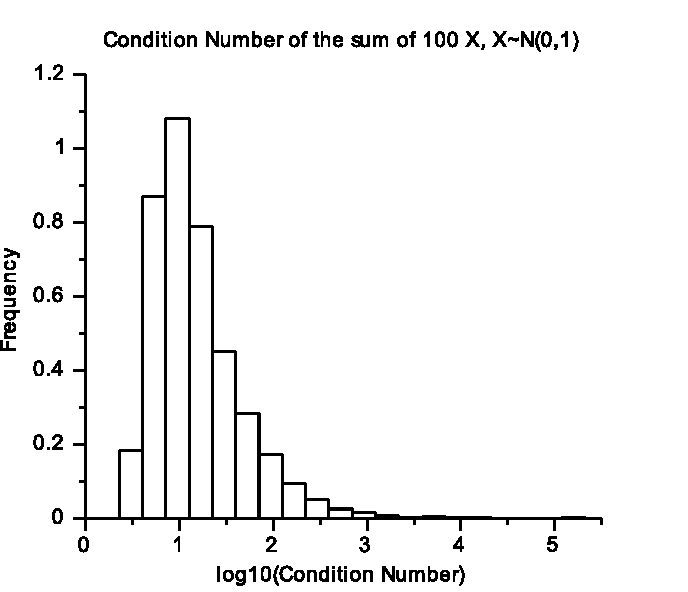
\includegraphics[width=\textwidth]{cond-sum-xnorm}
% \end{center}

	% \end{columns}

% \end{frame}

% %%%%%%%%%%%%%%%%%%%%%%%%%%%%%%%%%%%%%%%%%%%%%%%%%%%%%%%%%%%%%%%%%%%%%%%%%%%%%
% \begin{frame}[containsverbatim]
% \frametitle{Moyenne - partie 1 : analyse du conditionnement}

% On a $\epsilon_M\approx 10^{-15}$ et on suppose que $c\approx 10$. 

% Je prends \sciobj{reltol}$\approx 10^{-14}$.

% Test (naïf) :
% \begin{lstlisting}
% grand("setsd",0)
% x=grand(1000,1,"unf",0,1)
% y=G(x)
% computed=mean(y)
% expected=0.5
% reltol=1e-14 // <- Nouveau
% assert_checkalmostequal(computed,expected,reltol)
% \end{lstlisting}

% Problèmes :
% \begin{itemize}
% \item $10^{-14}$ pourrait être trop exigeant pour certaines 
% sommes très mal conditionnées.
% \item En général, l'erreur d'estimation est plus grande que 
% l'erreur de conditionnement.
% \end{itemize}

% \end{frame}
%%%%%%%%%%%%%%%%%%%%%%%%%%%%%%%%%%%%%%%%%%%%%%%%%%%%%%%%%%%%%%%%%%%%%%%%%%%%%
\begin{frame}[containsverbatim]
\frametitle{Moyenne - partie 2 : analyse probabiliste}

Supposons que 
$$
Y\sim \mathcal{N}(\mu,\sigma^2).
$$
et estimons l'espérance par la moyenne empirique.

Si $\mu=0$ :
\begin{itemize}
\item problème mal conditionné.
\item $y_i$ de signes différents, 
certaines d'entre elles étant de grande amplitude (mais elles sont 
rares).
\end{itemize}

Si $\mu\approx 1$ :
\begin{itemize}
\item problème probablement bien conditionné.
\item la plupart des $y_i$ sont positifs.
\end{itemize}

\end{frame}

%%%%%%%%%%%%%%%%%%%%%%%%%%%%%%%%%%%%%%%%%%%%%%%%%%%%%%%%%%%%%%%%%%%%%%%%%%%%%

\begin{frame}[containsverbatim]
\frametitle{Moyenne - partie 2 : analyse probabiliste}

Conséquences :
\begin{itemize}
\item Si $\mu=0$ : erreur absolue (somme mal conditionnée). 
\item Si $\mu\approx 1$ : erreur relative et 
le conditionnement est souvent raisonnable. 
\end{itemize}

Analyse :
\begin{itemize}
\item Il peut être souhaitable d'utiliser un algorithme très précis.
\item D'un autre côté, en général, l'intervalle de confiance sur 
$M_n$ est souvent beaucoup plus large que l'erreur dûe au 
conditionnement (voir la suite). 
\end{itemize}

\end{frame}

%%%%%%%%%%%%%%%%%%%%%%%%%%%%%%%%%%%%%%%%%%%%%%%%%%%%%%%%%%%%%%%%%%%%%%%%%%%%%

\begin{frame}[containsverbatim]
\frametitle{Moyenne - partie 2 : analyse probabiliste}

On note :
$$
S_n^2 = \frac{1}{n} \sum_{i=1}^n (y_i-M_n)^2
$$
l'écart-type empirique biaisé.

Si $n\gtrsim 100$, alors 
$$
P\left( M_n - z_{1-\alpha/2} \frac{S_n}{\sqrt{n-1}} \leq \mu 
\leq M_n + z_{1-\alpha/2} \frac{S_n}{\sqrt{n-1}} \right) \simeq 1-\alpha,
$$
où $z_{1-\alpha/2}$ est le quantile de niveau $1-\alpha/2$ de la loi Normale standard.

Exemple : $\alpha=0.05$ 
$$
P\left( M_n - 1.96 \frac{S_n}{\sqrt{n-1}} \leq \mu 
\leq M_n + 1.96 \frac{S_n}{\sqrt{n-1}} \right) \simeq 0.95.
$$

Interprétation pour la validation :
utiliser une erreur absolue.

\end{frame}

%%%%%%%%%%%%%%%%%%%%%%%%%%%%%%%%%%%%%%%%%%%%%%%%%%%%%%%%%%%%%%%%%%%%%%%%%%%%%
\begin{frame}[containsverbatim]
\frametitle{Tester un calcul probabiliste}

Test :
\begin{lstlisting}
grand("setsd",0)
n=1000
x=grand(n,1,"unf",0,1)
y=G(x)
computed=mean(y)
expected=0.5
abstol=1.96*st_deviation(y)/sqrt(n-1)  // <- Nouveau
assert_checkalmostequal(computed,expected,[],abstol)
\end{lstlisting}

Avantages :
\begin{itemize}
\item La tolérance absolue dépend de la valeur qu'on estime. 
\item Le test passe pour 95\% des graînes. 
\item Le test est peu sensible au générateur. 
\end{itemize}

Inconvénient :
\begin{itemize}
\item Il faut l'écart-type exact (ou bien une 
estimation).
\item Il peut être nécessaire d'ajuster la graîne pour 
faire passer le test.
\end{itemize}

\end{frame}

%%%%%%%%%%%%%%%%%%%%%%%%%%%%%%%%%%%%%%%%%%%%%%%%%%%%%%%%%%%%%%%%%%%%%%%%%%%%%
\begin{frame}[containsverbatim]
\frametitle{Aller plus loin}

Pour aller plus loin, on pourrait 
\begin{itemize}
\item tester la distribution des réalisations $y_i$
\item répéter l'expérience et comparer la distribution des réalisations $M_n$ 
avec la loi normale issue du TCL
\end{itemize}

Si on voulait tester le générateur de nombres pseudo-aléatoires :
\begin{itemize}
\item comparaison de la distribution des $U_n$ avec la distribution 
uniforme théorique
\item technique : tests statistiques (par exemple : test du $\chi^2$ ou 
Kolmogorov-Smirnov).
\end{itemize}

(Autre exemple pour les probabilités :  
\begin{itemize}
\item probabilité et probabilité complémentaire.)
\end{itemize}

\end{frame}

%%%%%%%%%%%%%%%%%%%%%%%%%%%%%%%%%%%%%%%%%%%%%%%%%%%%%%%%%%%%%%%%%%%%%%%%%%%%%

\section{Conclusion}

\begin{frame}
\frametitle{Conclusion}

\begin{itemize}
\item Pour tester un logiciel de calcul, connaître la 
différence entre un réel mathématique et un nombre à virgule 
flottante est utile. 
\item Une petite erreur relative en entrée $X$ peut être amplifiée par un 
mauvais conditionnement, d'où une grande erreur relative en sortie $Y$. 
\item Utiliser une librairie d'assertions prenant en compte 
les erreurs relatives ou absolues permet de vérifier des calculs 
numériques. 
\item On peut valider des calculs probabilistes, en vérifiant les propriétés 
des estimateurs statistiques qu'on calcule.
\end{itemize}

\end{frame}

%%%%%%%%%%%%%%%%%%%%%%%%%%%%%%%%%%%%%%%%%%%%%%%%%%%%%%%%%%%%%%%%%%%%%%%%%%%%%

\begin{frame}
\frametitle{Bibliographie}

\begin{itemize}
\item "Accuracy and stability of numerical algorithms", N. Higham, 2002, 
Society for Industrial and Applied Mathematics
\item "Using Accurate Arithmetics to Improve Numerical 
Reproducibility and Stability in Parallel Applications", 
Yun He and Chris H.Q. Ding. Journal of Supercomputing, 
Vol.18, Issue 3, 259-277, March 2001.
\item "Handbook of Floating Point Computations", 
J.-M. Muller, N. Brisebarre, F. de Dinechin, C.-P. Jeannerod, 
V. Lefèvre, G. Melquiond, N. Revol, D. Stehlé, S. Torres, 2010, 
Birkhäuser Basel.
\item "Afternotes on numerical analysis", G.W. Stewart, 1996, 
Lecture 7 "Computing sums"
\end{itemize}
  
\end{frame}

%%%%%%%%%%%%%%%%%%%%%%%%%%%%%%%%%%%%%%%%%%%%%%%%%%%%%%%%%%%%%%%%%%%%%%%%%%%%%

\begin{frame}
\frametitle{Bibliographie}

\begin{itemize}
\item "Open Source and Traditional Technical Computing", 
Alan Edelman, Massachusetts Institute of Technology, 
Scilabtec10, June 16, 2010
\item "Testing Math Functions in Microsoft Cloud Numerics", 
Stuart Brorson, Alan Edelman, Ben Moskowitz, 
MSDN Magazine, October 2012
\item Eddins, "Automated Software Testing for MATLAB", 
Computing in Science \& Engineering, 2009
\end{itemize}
  
\end{frame}

%%%%%%%%%%%%%%%%%%%%%%%%%%%%%%%%%%%%%%%%%%%%%%%%%%%%%%%%%%%%%%%%%%%%%%%%%%%%%

\begin{frame}
\frametitle{Bibliographie}

\begin{itemize}
\item A comparative study of the reliability of nine statistical 
software packages, Kellie B. Keeling, Robert J. Pavur, 
Computational Statistics \& Data Analysis 51 (2007), 3811 – 3831
\item Assessing the Reliability of Statistical Software: Part I, 
B. D. McCullough, The American Statistician, Vol. 52, 
No. 4 (Nov., 1998), pp. 358-366
\item Assessing the Reliability of Statistical Software: Part II
B. D. McCullough, The American Statistician, Vol. 53, 
No. 2 (May, 1999), pp. 149-159
\item Fixing statistical errors in spreadsheet software : the 
case of Gnumeric and Excel, B.D. Mc Cullough, 2004
\item The accuracy of statistical distributions in Microsoft 
Excel 2007, A. Talha Yalta, Computational Statistics and Data Analysis, 
 52 (2008) 4579-4586
\end{itemize}
  
\end{frame}

%%%%%%%%%%%%%%%%%%%%%%%%%%%%%%%%%%%%%%%%%%%%%%%%%%%%%%%%%%%%%%%%%%%%%%%%%%%%%

\begin{frame}

Merci de votre attention !

Questions ?
  
\end{frame}

%%%%%%%%%%%%%%%%%%%%%%%%%%%%%%%%%%%%%%%%%%%%%%%%%%%%%%%%%%%%%%%%%%%%%%%%%%%%%

\section{Annexes}

\begin{frame}

\begin{center}
ANNEXES
\end{center}
  
\end{frame}

%%%%%%%%%%%%%%%%%%%%%%%%%%%%%%%%%%%%%%%%%%%%%%%%%%%%%%%%%%%%%%%%%%%%%%%%%%%%%
\subsection{Flottants : détails}

\begin{frame}
\frametitle{Flottants : détails}
  \begin{columns}
    \column{0.5\textwidth}
    
    \column{0.5\textwidth}
    {\usebeamercolor[fg]{title}\huge{Flottants : détails}}
	
	Bit implicite, flottants extrêmes et conditionnement 
	d'une fonction réelle.
  \end{columns}
\end{frame}

%%%%%%%%%%%%%%%%%%%%%%%%%%%%%%%%%%%%%%%%%%%%%%%%%%%%%%%%%%%%%%%%%%%%%%%%%%%%%
%\subsection{Flottants normalisés, dénormalisés}

\begin{frame}
\frametitle{Nombres flottants}

Unicité de la représentation ? Je divise $M$ par 2, j'ajoute 1 à $e$.

Donc la définition précédente ne garantit pas l'unicité de la représentation. 


\begin{theorem}
(\emph{Flottant normalisé})
Un flottant est normalisé si $M$ satisfait :
$$
\beta^{p-1} \leq |M| < \beta^p.
$$
Si $x$ est un flottant normalisé non nul, alors sa représentation $(M,e)$ 
est unique et 
$$
e = \lfloor \log_\beta(|x|) \rfloor, \qquad 
M = \frac{x}{\beta^{e-p+1}}.
$$
\end{theorem}

\emph{Pour obtenir l'unicité, on ajoute une borne sur $M$.}

\end{frame}

%%%%%%%%%%%%%%%%%%%%%%%%%%%%%%%%%%%%%%%%%%%%%%%%%%%%%%%%%%%%%%%%%%%%%%%%%%%%%

\begin{frame}
\frametitle{Nombres flottants dénormalisés}

\begin{definition}
(\emph{Flottant dénormalisé})
Un flottant $(M,e)$ est dénormalisé si $e=e_{min}$ et $M$ satisfait :
$$
|M| < \beta^{p-1}
$$
\end{definition}

En anglais : \emph{subnormal}.

\end{frame}

%%%%%%%%%%%%%%%%%%%%%%%%%%%%%%%%%%%%%%%%%%%%%%%%%%%%%%%%%%%%%%%%%%%%%%%%%%%%%

%\subsection{Bit implicite}

%%%%%%%%%%%%%%%%%%%%%%%%%%%%%%%%%%%%%%%%%%%%%%%%%%%%%%%%%%%%%%%%%%%%%%%%%%%%%

\begin{frame}
\frametitle{Nombres flottants}

En base $\beta=2$ :
\begin{itemize}
\item Si $x$ normalisé :
$x = \pm  (1 . d_2\cdots d_p)_2 \cdot 2^e$,
\item Si $x$ dénormalisé :
$x = \pm  (0 . d_2\cdots d_p)_2 \cdot 2^e$.
\end{itemize}

Dans le standard IEEE 754-2008 :
\begin{itemize}
\item Un encodage particulier de 
l'exposant permet de savoir si $x$ est normalisé ou dénormalisé.
\item Le bit $d_1$ est donc stocké de manière \emph{implicite}. 
\item Cela explique pourquoi les doubles sont associés à la précision $p=53$, 
alors que seulement 52 bits sont stockés.
\end{itemize}

\end{frame}

%%%%%%%%%%%%%%%%%%%%%%%%%%%%%%%%%%%%%%%%%%%%%%%%%%%%%%%%%%%%%%%%%%%%%%%%%%%%%

\begin{frame}
\frametitle{Nombres flottants}

\begin{example}
Considérons le système flottant jouet de base $\beta=2$, de précision $p=3$ et 
d'amplitude d'exposants $e_{min}=-2$ et $e_{max}=3$. 

Le nombre réel $x=3$ peut être représenté par le nombre flottant 
$(M,e)=(6,1)$ :
\begin{eqnarray}
x = 6 \cdot 2^{1-3+1} = 6 \cdot 2^{-1} = 3.
\end{eqnarray}
Vérifions les équations. 
La partie intégrale $M$ satisfait 
$$
|M|=6\leq \beta^p-1=2^3-1 = 7
$$
et l'exposant $e$ satisfait 
$$
-2 \leq e \leq 3
$$
\end{example}

\end{frame}

%%%%%%%%%%%%%%%%%%%%%%%%%%%%%%%%%%%%%%%%%%%%%%%%%%%%%%%%%%%%%%%%%%%%%%%%%%%%%

\begin{frame}
\frametitle{Nombres flottants}

\begin{example}
Même système flottant "jouet" : $(\beta,p,e_{min},e_{max})=(2,3,-2,3)$.

Les nombres flottants normalisés sont tels que :
$$
\beta^{p-1}=4\leq |M| < \beta^p=8.
$$
\end{example}

Exercice : montrer que $(M,e)=(6,1)$ est le flottant normalisé pour $x=3$, 
et que $(M,e)=(3,2)$ ne l'est pas.

\end{frame}

%%%%%%%%%%%%%%%%%%%%%%%%%%%%%%%%%%%%%%%%%%%%%%%%%%%%%%%%%%%%%%%%%%%%%%%%%%%%%

\begin{frame}
\frametitle{Nombres flottants}

\begin{example}
Même système flottant "jouet" : $(\beta,p,e_{min},e_{max})=(2,3,-2,3)$.

On considère $x=0.125$. 
On trouve :
$$
\lfloor \log_\beta(|x|) \rfloor = -3
$$
qui est plus petit que $e_{min}=-2$. 
Le nombre est dénormalisé. 
On met $e=-2$ et on calcule :
$$
M = \frac{x}{\beta^{e-p+1}} = 2
$$
On trouve que $M$ est un entier. 
Donc le couple $(M,e)=(2,-2)$ est une représentation dénormalisée 
de $x=0.125$ dans ce système.
\end{example}

\end{frame}

%%%%%%%%%%%%%%%%%%%%%%%%%%%%%%%%%%%%%%%%%%%%%%%%%%%%%%%%%%%%%%%%%%%%%%%%%%%%%
\begin{frame}
\frametitle{Nombres réels en base $\beta$}

\begin{theorem}
(\emph{Représentation d'un réel en base $\beta$})
Supposons que $x$ est un flottant. 
Alors, le nombre $x$ peut être écrit sous la forme :
$$
x = \pm \left( 
d_1
+ \frac{d_2}{\beta} + \ldots 
+ \frac{d_p}{\beta^{p-1}} \right) \cdot \beta^e, 
$$
ou encore:
$$
x = \pm  (d_1 . d_2\cdots d_p)_\beta \cdot \beta^e.
$$
avec $d_1,...,d_p\in\{0,1,...,b-1\}$.
\end{theorem}

Exercice : faire la preuve.

Idée : décomposer $|M|$ sous la forme :
$$
|M|=d_1\beta^{p-1} + d_2\beta^{p-2} + \ldots + d_p.
$$

\end{frame}

%%%%%%%%%%%%%%%%%%%%%%%%%%%%%%%%%%%%%%%%%%%%%%%%%%%%%%%%%%%%%%%%%%%%%%%%%%%%%

\begin{frame}
\frametitle{Nombres flottants}
\begin{theorem}
(\emph{Bit de tête de la représentation en base $\beta$})
Supposons que $x$ est un flottant. 
\begin{itemize}
\item Si $x$ est normalisé, alors $d_1\neq 0$.
\item Si $x$ est dénormalisé, alors $d_1=0$.
\end{itemize}
\end{theorem}

Exercice : preuve.

\end{frame}

%%%%%%%%%%%%%%%%%%%%%%%%%%%%%%%%%%%%%%%%%%%%%%%%%%%%%%%%%%%%%%%%%%%%%%%%%%%%%

\begin{frame}
\frametitle{Nombres flottants}

Les flottants positifs (normalisés et dénormalisés) dans le système "jouet" : $(\beta,p,e_{min},e_{max})=(2,3,-2,3)$.

\begin{center}
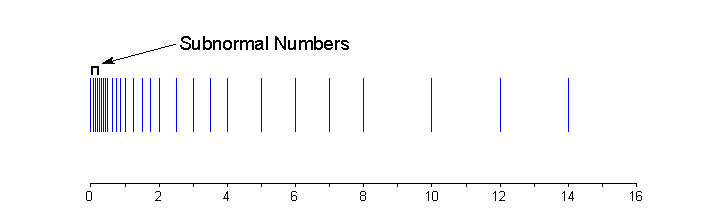
\includegraphics[width=0.9\textwidth]{toysystem_positive}
\end{center}

\end{frame}

%%%%%%%%%%%%%%%%%%%%%%%%%%%%%%%%%%%%%%%%%%%%%%%%%%%%%%%%%%%%%%%%%%%%%%%%%%%%%
\begin{frame}
\frametitle{Nombres flottants extrêmes}

\begin{theorem}
(\emph{Flottants extrêmes})
Considérons le système flottant $\beta$, $p$, $e_{min}$, $e_{max}$.
\begin{itemize}
\item Le plus petit flottant normalisé est
$$
\mu = \beta^{e_{min}}.
$$

\item Le plus grand flottant normalisé est 
$$
\Omega = (\beta - \beta^{1-p}) \beta^{e_{max}}.
$$

\item Le plus petit flottant dénormalisé est 
$$
\alpha = \beta^{e_{min}-p+1}.
$$
\end{itemize}
\end{theorem}

\end{frame}

%%%%%%%%%%%%%%%%%%%%%%%%%%%%%%%%%%%%%%%%%%%%%%%%%%%%%%%%%%%%%%%%%%%%%%%%%%%%%

\begin{frame}
\frametitle{Conditionnement}

Preuve :

Par définition, on a :
$$
K_G(x)
= \lim_{\Delta x \rightarrow 0} \left| \frac{\frac{\hat{y} - y}{y}}{\frac{\hat{x} - x}{x}}\right|
$$
La formule de Taylor :
$$
f(x+\Delta x) = f(x) + f^\prime(x)\Delta x 
		+ O((\Delta x)^2)
$$
implique
$$
\frac{\hat{y} - y}{y}
= \frac{f(x+\Delta x) - f(x)}{f(x)} 
= \frac{f^\prime(x)\Delta x + O((\Delta x)^2)}{f(x)}.
$$
\end{frame}

%%%%%%%%%%%%%%%%%%%%%%%%%%%%%%%%%%%%%%%%%%%%%%%%%%%%%%%%%%%%%%%%%%%%%%%%%%%%%

\begin{frame}
\frametitle{Conditionnement}

Donc:
\begin{eqnarray}
\left| \frac{E_{rel}(y,\hat{y})}{E_{rel}(x,\hat{x})}\right|
&=& \left| \frac{\frac{f^\prime(x)\Delta x + O((\Delta x)^2)}{f(x)}}{\frac{\Delta x}{x}}\right| \\
&=& \left| \frac{x}{\Delta x} \frac{f^\prime(x)\Delta x + O((\Delta x)^2)}{f(x)}\right| \\
&=& \left| \frac{x}{f(x)} (f^\prime(x) + O(\Delta x)\right|
\end{eqnarray}
Pour conclure, on prend $\Delta x \rightarrow 0$. 

\end{frame}

%%%%%%%%%%%%%%%%%%%%%%%%%%%%%%%%%%%%%%%%%%%%%%%%%%%%%%%%%%%%%%%%%%%%%%%%%%%%%

\begin{frame}
\frametitle{Conditionnement}

Conditionnement de $\log(x)$ quand $x\rightarrow 1$:

\begin{center}
\begin{tabular}{lll}
$x$ & $\log(x)$ & $K(x)$ \\
\hline
1.01 & 0.00995033085317 & 100.499170807\\
1.0001 & 9.99950003333e-05 & 10000.4999917 \\
1.000001 & 9.99999499918e-07 & 1000000.50008\\
\end{tabular}
\end{center}

\end{frame}

%%%%%%%%%%%%%%%%%%%%%%%%%%%%%%%%%%%%%%%%%%%%%%%%%%%%%%%%%%%%%%%%%%%%%%%%%%%%%

\begin{frame}
\frametitle{Erreur d'évaluation}

\begin{theorem}
(\emph{Erreur relative des opérations algébriques.})
Soit $x$ et $y$ des doubles. 
Les opérations arithmétiques +,-,*,/ satisfont:
$$
fl(x \; op \; y)=(x\; op\; y) (1+\delta),
$$
où
$$
|\delta|\leq u.
$$
\end{theorem}

\emph{L'erreur relative sur $x\; op\; y$ est inférieure à $u$ 
pour les opérations algébriques.}

\end{frame}

%%%%%%%%%%%%%%%%%%%%%%%%%%%%%%%%%%%%%%%%%%%%%%%%%%%%%%%%%%%%%%%%%%%%%%%%%%%%%

\begin{frame}
\frametitle{Erreur relative, absolue}

% Source : Accuracy and stability of numerical algorithms.

\begin{theorem}
(\emph{Erreur relative (2ième définition)})
Supposons que $x$ et $\hat{x}$ sont deux réels différents de zéro. 
Alors il existe un réel $\rho$ tel que :
$$
E_{rel}(x,\hat{x}) = |\rho|
$$
avec 
$$
\hat{x} = x(1+\rho).
$$
\end{theorem}

\begin{proof}
On a $\hat{x} = x + \rho x$, donc :
$$
\frac{\hat{x}-x}{x} = \rho.
$$
La réciproque est triviale.
\end{proof}

\end{frame}

%%%%%%%%%%%%%%%%%%%%%%%%%%%%%%%%%%%%%%%%%%%%%%%%%%%%%%%%%%%%%%%%%%%%%%%%%%%%%

\begin{frame}
\frametitle{Erreur relative, absolue}

% Source : Accuracy and stability of numerical algorithms.

\begin{theorem}
(\emph{Invariance par rapport à un changement d'échelle.})
On suppose que $x$, $\hat{x}$ sont différents de zéro.
Soit $\alpha>0$ un réel représentant un facteur de changement d'échelle. 
On considère 
$$
x^\prime=\alpha x, \quad \hat{x}^\prime=\alpha \hat{x}.
$$
Alors 
$$
E_{rel}(x,\hat{x}) = E_{rel}(x^\prime,\hat{x}^\prime)
$$
\end{theorem}

\emph{L'erreur relative est inchangée par changement d'échelle.}

\end{frame}

%%%%%%%%%%%%%%%%%%%%%%%%%%%%%%%%%%%%%%%%%%%%%%%%%%%%%%%%%%%%%%%%%%%%%%%%%%%%%
\subsection{Testabilité}

\begin{frame}
\frametitle{Testabilité}
  \begin{columns}
    \column{0.5\textwidth}
    
    \column{0.5\textwidth}
    {\usebeamercolor[fg]{title}\huge{Testabilité}}
	
	Améliorer la testabilité d'une fonction, 
	la notion de privé/public pour gérer les tests. 
  \end{columns}
\end{frame}

%%%%%%%%%%%%%%%%%%%%%%%%%%%%%%%%%%%%%%%%%%%%%%%%%%%%%%%%%%%%%%%%%%%%%%%%%%%%%

\begin{frame}[containsverbatim]
\frametitle{\emph{"Tester, c'est impossible !"}}

\begin{itemize}
\item En général, une fonction qui n'est pas testable ne devrait pas 
être fournie à un utilisateur.
\item Au contraire, la fonction doit être conçue pour être facile à 
tester. 
\end{itemize}

Deux cas :
\begin{itemize}
\item Si l'entrée a une influence mesurable sur la sortie, alors 
la fonction est testable.
\item Sinon la fonction n'est pas testable. 
\end{itemize}

Exemple de fonction non testable : l'appel à la fonction est 
sous la forme :
$$
G()
$$
et met à jour un état interne caché à l'utilisateur. 

Exemple : bouton "mise à jour" d'une interface graphique, sans 
aucun changement de l'état externe.

\end{frame}

%%%%%%%%%%%%%%%%%%%%%%%%%%%%%%%%%%%%%%%%%%%%%%%%%%%%%%%%%%%%%%%%%%%%%%%%%%%%%

\begin{frame}[containsverbatim]
\frametitle{\emph{"Tester, c'est impossible !"}}
Si la fonction n'est pas testable, que faire ?
\begin{itemize}
\item Mieux choisir les entrées. 
Exemple : ajouter des entrées cachées du code pour le 
rendre testable (\emph{certains} - mais pas tous - 
paramètres algorithmiques \emph{en dur} : pas de discrétisation $h$, 
nombre d'itérations, maximal, etc...).
\item Mieux choisir la fonction. 
Exemple : découper une fonction globale en plusieurs 
sous-fonctions pour pouvoir tester des parties de l'algorithme.
\item Mieux choisir les sorties. 
Exemple : ajouter des sorties cachées au code pour le rendre testable. 
\end{itemize}

Exemple :
\begin{itemize}
\item Pouvoir définir le pas de discrétisation $h$ 
permet de tester la convergence d'une méthode de différences 
finies lorsque $h\rightarrow 0$.
\end{itemize}

\end{frame}

%%%%%%%%%%%%%%%%%%%%%%%%%%%%%%%%%%%%%%%%%%%%%%%%%%%%%%%%%%%%%%%%%%%%%%%%%%%%%

\begin{frame}[containsverbatim]
\frametitle{Jusqu'où tester ?}

Une \emph{fonctionnalité} est un couple $(X,G)$, où $X$ est dans 
un certain espace des paramètres possibles (par exemple : $X_1\in[0,1]$, 
$X_1=0,1,...,4$, etc...).

Objectif : 
$$
\textrm{nombre de tests }\geq C \times \textrm{ nombres de fonctionnalités}, 
$$
où $C\geq 1$ est la plus petite constante possible.

\emph{"Ma librairie a $10^6$ fonctionnalités différentes. Je 
dois faire $10^6$ tests ?"}

En général, beaucoup moins : on ne teste que 
\begin{itemize}
\item ce que l'utilisateur modifie en entrée $X$,
\item les fonctions $G$ que l'utilisateur peut manipuler, 
\item ce que l'utilisateur "voit" en sortie $Y$.
\end{itemize}

\end{frame}

%%%%%%%%%%%%%%%%%%%%%%%%%%%%%%%%%%%%%%%%%%%%%%%%%%%%%%%%%%%%%%%%%%%%%%%%%%%%%

\begin{frame}[containsverbatim]
\frametitle{Jusqu'où tester ?}

Principes :
\begin{itemize}
\item Economie : pourquoi tester une fonction 
invisible de l'utilisateur (privée) ?
\item Confiance: pourquoi fournir à l'utilisateur 
une fonction (publique) non testée ?
\end{itemize}

Exemples :
\begin{itemize}
\item les états d'une interface graphique (p.ex.:allumé/éteint), 
\item les valeurs dans un fichier de sortie.
\end{itemize}
\end{frame}

%%%%%%%%%%%%%%%%%%%%%%%%%%%%%%%%%%%%%%%%%%%%%%%%%%%%%%%%%%%%%%%%%%%%%%%%%%%%%

\begin{frame}[containsverbatim]
\frametitle{Jusqu'où tester ?}

Conséquences :
\begin{itemize}
\item Limiter ce que "voit" l'utilisateur en entrée 
ou en sortie permet de limiter les tests : notion de privé/publique 
dans les langages de programmation.
\item A l'extrême, l'unique fonction facile à tester n'a aucune entrée 
et aucune sortie $G()$. Problème : la fonction n'est plus utilisable !
\item En pratique, compromis entre testabilité et utilisabilité :
\begin{center}
\emph{Compte tenu de l'effort à fournir pour 
tester une fonctionnalité, est-ce possible de la rendre publique ?}
\end{center}
\end{itemize}

\end{frame}

%%%%%%%%%%%%%%%%%%%%%%%%%%%%%%%%%%%%%%%%%%%%%%%%%%%%%%%%%%%%%%%%%%%%%%%%%%%%%

\begin{frame}[containsverbatim]
\frametitle{Jusqu'où tester ?}

\begin{center}
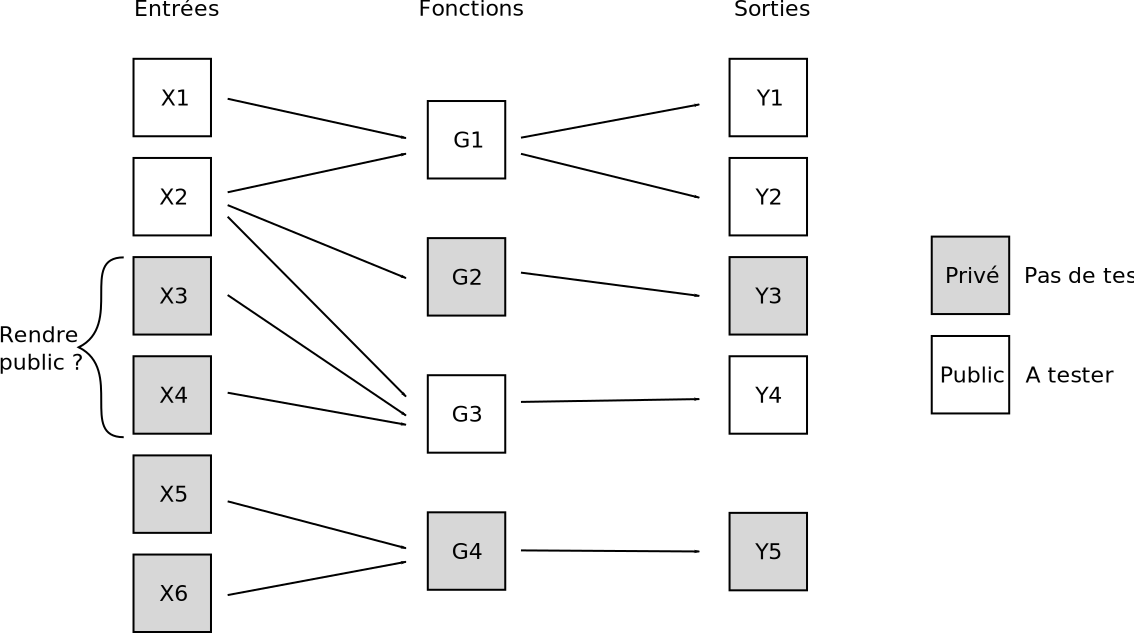
\includegraphics[width=\textwidth]{publique-prive}
\end{center}

\end{frame}

%%%%%%%%%%%%%%%%%%%%%%%%%%%%%%%%%%%%%%%%%%%%%%%%%%%%%%%%%%%%%%%%%%%%%%%%%%%%%

\subsection{Combinatoire}

\begin{frame}
\frametitle{Combinatoire}
  \begin{columns}
    \column{0.5\textwidth}
    
    \column{0.5\textwidth}
    {\usebeamercolor[fg]{title}\huge{Combinatoire}}
	
	Limiter le nombre de combinaisons d'options à tester, 
	choisir ses expériences selon un plan.
  \end{columns}
\end{frame}

%%%%%%%%%%%%%%%%%%%%%%%%%%%%%%%%%%%%%%%%%%%%%%%%%%%%%%%%%%%%%%%%%%%%%%%%%%%%%

\begin{frame}
\frametitle{\emph{"Impossible de tester avec toutes ces combinaisons!"}}

\emph{"Ma fonction a $10$ options binaires différentes. Je 
dois faire $2^{10}$ tests ?"}

\begin{center}
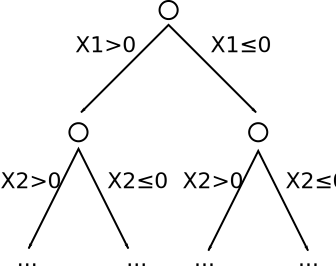
\includegraphics[width=0.4\textwidth]{combinatoire}
\end{center}

A minima, 10 tests suffisent car :
\begin{itemize}
\item on peut \emph{factoriser} le code source pour regrouper 
les branches de l'arbre combinatoire,
\item la plupart du temps, le développeur est suffisamment 
"économe" (ou flemmard ?) pour écrire un code 
factorisé.
\end{itemize}
\end{frame}

%%%%%%%%%%%%%%%%%%%%%%%%%%%%%%%%%%%%%%%%%%%%%%%%%%%%%%%%%%%%%%%%%%%%%%%%%%%%%

\begin{frame}[containsverbatim]
\frametitle{Limiter la combinatoire}

\begin{example}
\begin{columns}[t]

% Column #1
    \begin{column}[t]{0.45\textwidth}
	
On ne dit pas :
\begin{lstlisting}
if (x1>0)&(x2>0) 
      // Cas 1
elseif (x1>0)&(x2<=0) 
      // Cas 2
elseif (x1<=0)&(x2>0) 
      // Cas 3
elseif (x1<=0)&(x2<=0) 
      // Cas 4
end
\end{lstlisting}

    \end{column}
	
% Column #2
    \begin{column}[t]{0.45\textwidth}

On dit (quand c'est possible) :
\begin{lstlisting}
if (x1>0) 
      // Cas 1
else
      // Cas 2
end
if (x2>0) 
      // Cas 3
else
      // Cas 4
end
\end{lstlisting}
    \end{column}
\end{columns}
Car : 
\begin{itemize}
\item le premier bloc \pyobj{if} est exécuté quelque soit \pyobj{x2},
\item le second bloc \pyobj{if} est exécuté quelque soit \pyobj{x1}.
\end{itemize}
\end{example}

\end{frame}
%%%%%%%%%%%%%%%%%%%%%%%%%%%%%%%%%%%%%%%%%%%%%%%%%%%%%%%%%%%%%%%%%%%%%%%%%%%%%

\begin{frame}[containsverbatim]
\frametitle{Limiter la combinatoire}

\begin{example}
On suppose qu'on a 2 options avec 4 niveaux. 

Quelles expériences $(x_1,x_2)$ doit-on réaliser ?
\begin{columns}[t]

% Column #1
    \begin{column}[t]{0.25\textwidth}
Full factorial : 

$E=16$

\begin{tabular}{l|l}
(1,1)&(3,1)\\
(1,2)&(3,2)\\
(1,3)&(3,3)\\
(1,4)&(3,4)\\
\hline
(2,1)&(4,1)\\
(2,2)&(4,2)\\
(2,3)&(4,3)\\
(2,4)&(4,4)\\
\end{tabular}

    \end{column}
	
% Column #2
    \begin{column}[t]{0.25\textwidth}
One at a time : 

$E=8$

\begin{tabular}{l}
(1,1)\\
(2,1)\\
(3,1)\\
(4,1)\\
\hline
(1,1)\\
(1,2)\\
(1,3)\\
(1,4)\\
\end{tabular}

    \end{column}
% Column #3
    \begin{column}[t]{0.25\textwidth}
Diagonal : 

$E=4$

\begin{tabular}{l}
(1,1)\\
(2,2)\\
(3,3)\\
(4,4)\\
\end{tabular}

    \end{column}
\end{columns}

\end{example}

\end{frame}
%%%%%%%%%%%%%%%%%%%%%%%%%%%%%%%%%%%%%%%%%%%%%%%%%%%%%%%%%%%%%%%%%%%%%%%%%%%%%

\begin{frame}[containsverbatim]
\frametitle{Lorsque les options de $G$ ne sont plus binaires}

Supposons que les $n$ variables d'entrée discrèetes ont $m$ niveaux. 
Combien d'expériences $E$ ?
\begin{itemize}
\item A minima, $E=m$ tests pour un plan "Diagonal".
	\begin{itemize}
	\item Minimum possible d'expériences qui couvrent toutes 
	les options. 
	\end{itemize}
\item En général, $E=nm$ tests pour un plan "One At A Time".
	\begin{itemize}
	\item Chaque option est testée séparément, ce qui facilite l'écriture du test. 
	\end{itemize}
\item Au mieux, $E=n^m$ tests pour un plan "Full Factorial".
	\begin{itemize}
	\item Toutes les combinaisons sont couvertes. 
	\end{itemize}
\end{itemize}

\end{frame}
%%%%%%%%%%%%%%%%%%%%%%%%%%%%%%%%%%%%%%%%%%%%%%%%%%%%%%%%%%%%%%%%%%%%%%%%%%%%%

\begin{frame}[containsverbatim]
\frametitle{Moyenne - partie 2 : analyse probabiliste}

(No offense...)

On note :
$$
S_n^2 = \frac{1}{n} \sum_{i=1}^n (y_i-M_n)^2
$$
l'écart-type empirique biaisé.

\begin{theorem}
Supposons que $\{y_i\}_{i=1,\ldots,n}$ sont des réalisations indépendantes de 
loi $\mathcal{N}(\mu,\sigma^2)$. 
Alors :
$$
\frac{M_n-\mu}{S_n/\sqrt{n-1}} \sim \mathcal{T}_{n-1},
$$
où $\mathcal{T}_{n-1}$ est la loi de Student à $n-1$ 
degrés de liberté.
\end{theorem}

Dans le cas général, la loi de $Y$ est inconnue, 
et il n'est pas possible de calculer un intervalle de confiance 
sur $M_n$. 

\end{frame}

%%%%%%%%%%%%%%%%%%%%%%%%%%%%%%%%%%%%%%%%%%%%%%%%%%%%%%%%%%%%%%%%%%%%%%%%%%%%%

\begin{frame}[containsverbatim]
\frametitle{Moyenne - partie 2 : analyse probabiliste}

(No offense...)

\begin{theorem}
(\emph{Théorème central limite})
Supposons que $\{y_i\}_{i=1,\ldots,n}$ sont des réalisations indépendantes de 
même loi, de moyenne $\mu$ et de variance $\sigma^2$. 
Alors :
$$
\frac{1}{\sqrt{n}} \sum_{i=1}^n \frac{y_i-\mu}{\sigma} \rightarrow \mathcal{N}(0,1).
$$
\end{theorem}

De plus, lorsque $n$ est grand, la loi de Student converge vers la loi 
normale. 

\end{frame}

%%%%%%%%%%%%%%%%%%%%%%%%%%%%%%%%%%%%%%%%%%%%%%%%%%%%%%%%%%%%%%%%%%%%%%%%%%%%%

\begin{frame}
\frametitle{Conditionnement}

Le conditionnement 
\begin{itemize}
\item est une propriété du problème mathématique
\item n'est pas une propriété de la méthode numérique pour résoudre le problème
\end{itemize}

Le conditionnement mesure 
\begin{itemize}
\item l'amplification d'une erreur relative sur $x$
\item et son impact relatif sur $y$
\end{itemize}

Lorsque les calculs s'enchaînent, l'erreur peut 
\begin{itemize}
\item augmenter
\item diminuer
\end{itemize}
en fonction de:
\begin{itemize}
\item du conditionnement du problème mathématique
\item de la méthode numérique utilisée
\end{itemize}

\end{frame}

%%%%%%%%%%%%%%%%%%%%%%%%%%%%%%%%%%%%%%%%%%%%%%%%%%%%%%%%%%%%%%%%%%%%%%%%%%%%%

\begin{frame}
\frametitle{Erreur forward, backward}

\begin{definition}
(\emph{Backward stable})
Une méthode pour calculer $y=G(x)$ est backward stable si, pour 
tout $x$, elle produit une valeur $\hat{y}$ avec une petite erreur backward, 
c'est à dire telle que 
$$
\hat{y} = G(x+\Delta x)
$$
pour un $\Delta x$ "petit".
\end{definition}

La manière de définir "petit" dépend du contexte.

\end{frame}


\end{document}
